\documentclass[a4paper,fleql]{cas-sc}
\usepackage[authoryear,longnamesfirst]{natbib}
\usepackage{amsmath}
\usepackage{amssymb}
\DeclareMathAlphabet{\mathcal}{OMS}{cmsy}{m}{n}
\DeclareMathOperator*{\argmax}{arg\,max}
\usepackage{booktabs}
\usepackage{needspace}
\usepackage{graphicx}
\usepackage{algorithm}
\usepackage{algpseudocode}
\usepackage{multirow}
\usepackage{placeins}
\usepackage{float}
\usepackage{caption}
\usepackage{threeparttable}
\usepackage{tcolorbox}
\usepackage{xspace}

\makeatletter
\def\fps@figure{htbp}
\makeatother

\def\tsc#1{\csdef{#1}{\textsc{\lowercase{#1}}\xspace}}
\tsc{WGM}
\tsc{QE}

\begin{document}
\let\WriteBookmarks\relax
\def\floatpagepagefraction{0.7}
\def\textpagefraction{0.3}

\shorttitle{NexRoute: Dual-Axis Nexus Routing for LLMs}
\shortauthors{J. Kong, Y. Ha}

\title[mode=title]{NexRoute: A Dual-Axis Nexus Routing Framework for Adaptive
Expert Selection in Cross-Domain Large Language Models}

\tnotemark[1]
\tnotetext[1]{This work was supported by Konkuk University.}

\author[1]{Junyoung Kong}
\ead{junyoung.kong3162@konkuk.ac.kr}
\credit{Conceptualization, Methodology, Software, Writing -- original draft}

\author[1]{Youngguk Ha}%
\cormark[1]
\ead{ygha@konkuk.ac.kr}
\credit{Supervision, Writing -- review \& editing, Funding acquisition}

\cortext[1]{Corresponding author}

\affiliation[1]{%
    organization={Department of Computer Science and Engineering, Konkuk University},
    addressline={120 Neungdong-ro},
    city={Gwangjin-gu, Seoul},
    postcode={05029},
    country={Republic of Korea}
}

\begin{abstract}
Existing RAG-based expert systems route queries by domain identity alone,
ignoring the reasoning function required to process them. This functional
mismatch leads to cross-domain contamination and increased hallucination
under unified retrieval.
We propose \textbf{NexRoute}, a dual-axis routing framework that decomposes
each query along two orthogonal dimensions: a domain axis
(\texttt{LAW}, \texttt{MED}, \texttt{SOC}, \texttt{STEM}, \texttt{CROSS})
and a function axis (\texttt{What}, \texttt{How}, \texttt{Why},
\texttt{Compare}). Their intersection---the \textit{nexus point}---selects
the appropriate LoRA-based expert and applies a function-specific retrieval
scaffold, jointly addressing cross-domain contamination and functional
mismatch.
Trained on 15,744 dual-annotated MMLU samples, NexRoute 7B achieves
\textbf{87.4\%} routing accuracy (+2.2~pp over the strongest baseline),
a cross-domain BERTScore of \textbf{89.53} and ROUGE-L of \textbf{29.60}
($p < 0.05$, paired $t$-test on 500 samples)---both surpassing all
72B-scale dense baselines---and the lowest hallucination rate of
\textbf{8.9\%} among all 7B-scale models. These results demonstrate that
joint domain-function alignment is a significant driver of cross-domain
generation quality, independently of parameter scale.
\end{abstract}
\begin{highlights}
    \item NexRoute introduces dual-axis routing over domain and function
    axes, reducing functional mismatch in RAG-based multi-expert systems.
    \item A four-way function axis taxonomy \{\texttt{What}, \texttt{How},
    \texttt{Why}, \texttt{Compare}\} aligns LoRA expert activation with
    query reasoning intent.
    \item Domain-partitioned retrieval eliminates cross-domain contamination
    by construction, yielding the lowest hallucination rate of 8.9\% among
    all 7B-scale models (16.0\% relative reduction vs.\ Naive RAG 7B).
    \item NexRoute 7B achieves cross-domain BERTScore of 89.53 and
    ROUGE-L of 29.60, surpassing all tested 72B-scale dense baselines at
    $10\times$ fewer parameters ($p < 0.05$).
    \item The system operates within 14.8\,GB of GPU memory, enabling
    on-device deployment under data-privacy constraints.
\end{highlights}
\begin{keywords}
Retrieval-Augmented Generation \sep
Large Language Models \sep
Parameter-Efficient Fine-Tuning \sep
Expert Routing \sep
LoRA \sep
Domain Adaptation \sep
Cross-Domain Reasoning
\end{keywords}
\maketitle

%%==============================================================================
\section{Introduction}
\label{sec:introduction}
%%==============================================================================

LLMs are increasingly applied to professional domains such as legal
consultation and clinical decision support, where domain-specific accuracy
is essential \citep{brown2020gpt,touvron2023llama,singhal2023large}.
A dominant architectural approach combines domain-specialized LoRA adapters
with RAG pipelines to provide factual grounding without full fine-tuning
\citep{hu2022lora,shazeer2017outrageously,dou2024loramoe}. These frameworks,
however, route queries solely by domain identity, without modeling the
reasoning function the query demands.

Expert performance depends not only on \textit{which} knowledge domain is
relevant, but on \textit{how} that knowledge must be applied. A LoRA adapter
optimized for causal legal reasoning produces suboptimal responses when
activated for a definitional query in the same domain, because the reasoning
modality is mismatched to the query intent \citep{singhal2023large,guha2023legalbench}.
Furthermore, resolving complex interdisciplinary scenarios requires synergistic 
collaboration between distinct domain experts. Traditional architectures isolate 
a single expert module, forcing it to independently extract sparse contextual 
hints from massive information pools. In contrast, when specific specialized experts 
are explicitly paired, their combined reasoning frameworks unlock multi-faceted 
analytical pathways that neither could access alone. This targeted intersection 
drastically reduces the search space for relevant evidence, accelerating the overall 
deductive process. Ultimately, this structural synergy transforms fragmented information 
into highly accurate, diverse, and multidimensional resolutions.
However, in multi-domain settings, unified retrieval over undifferentiated corpora
further compounds this problem: lexical overlap between professional
disciplines causes the retriever to mix evidence from unrelated domains
(cross-domain contamination), as illustrated in Figure~\ref{fig:motivation}.

We propose \textbf{NexRoute}, which addresses both problems through
dual-axis routing. Each query is decomposed along two orthogonal dimensions:
(1) a \textbf{domain axis} (\texttt{LAW}, \texttt{MED}, \texttt{SOC},
\texttt{STEM}, \texttt{CROSS}) and (2) a \textbf{function axis}
(\texttt{What}, \texttt{How}, \texttt{Why}, \texttt{Compare}). Their
intersection---the \textit{nexus point}---determines which LoRA expert to
activate and which function-specific retrieval scaffold to apply, ensuring
that retrieved evidence aligns with the reasoning strategy the query demands.

\begin{center}
\includegraphics[width=\textwidth, height=0.85\textheight, keepaspectratio=true]{img1.png}
\end{center}
\begingroup
\captionof{figure}{Cross-domain contamination in unified-retrieval RAG
systems. Lexical ambiguity causes the retriever to fetch documents from an
unrelated domain (e.g., STEM passages for a MED query), polluting the
context window and inducing hallucination. NexRoute prevents this via
domain-partitioned retrieval (Section~\ref{sec:method}).}
\label{fig:motivation}
\endgroup

Our main contributions are as follows:
\begin{itemize}
    \item \textbf{Dual-axis routing architecture:} A joint domain-and-function
    classifier that simultaneously activates the appropriate LoRA expert and
    applies function-specific prompt scaffolding within a single synchronized
    step.

    \item \textbf{Function axis taxonomy:} A four-way reasoning taxonomy
    \{\texttt{What}, \texttt{How}, \texttt{Why}, \texttt{Compare}\}, jointly
    trained with domain classification over a shared DeBERTa-large encoder,
    building on type-aware query decomposition~\citep{typedrag}.

    \item \textbf{Cross-domain expert module:} A dedicated LoRA adapter
    trained on 1,321 synthesized domain-pair samples, enabling a compact
    7B model to handle multidisciplinary queries without merging
    single-domain adapters.

    \item \textbf{Cross-domain benchmark:} A 500-sample held-out evaluation
    set covering all five domain categories, including interdisciplinary
    scenarios not seen during training.

    \item \textbf{Empirical validation:} Experiments against four RAG
    baselines at 7B and 72B parameter scales demonstrate significant gains
    in routing accuracy, cross-domain generation quality, and hallucination
    suppression (Section~\ref{sec:experiments}).
\end{itemize}



The remainder of this paper is organized as follows.
Section~\ref{sec:related} reviews related work.
Section~\ref{sec:method} presents the NexRoute architecture.
Section~\ref{sec:experiments} reports quantitative results.
Section~\ref{sec:casestudy} presents the case study.
Section~\ref{sec:implementation} details implementation and hyperparameters.
Section~\ref{sec:discussion} discusses implications, and
Section~\ref{sec:conclusion} concludes the paper.
%%==============================================================================
\section{Related Work}
\label{sec:related}
%%==============================================================================

This section situates NexRoute within four interconnected research streams:
(1) Mixture-of-Experts architectures and their evolution toward sparse
specialization, (2) parameter-efficient fine-tuning for domain adaptation,
(3) retrieval-augmented generation and its structural limitations in
multi-domain settings, and (4) query routing strategies for intelligent expert
systems.

%%------------------------------------------------------------------------------
\subsection{Mixture-of-Experts for Intelligent Expert Systems}
%%------------------------------------------------------------------------------
The Mixture-of-Experts (MoE) paradigm \citep{shazeer2017outrageously} provides
a principled mechanism for conditional computation: rather than activating all
model parameters for every input, a learned gating network selectively routes
each token to a sparse subset of specialized feed-forward experts. This
selective activation strategy enables substantially larger model capacity
without proportional increases in inference cost, making MoE a natural
candidate for building scalable intelligent expert systems.

Fedus et al.\ \citep{fedus2022switch} simplified MoE routing to a top-1
selection strategy in Switch Transformer, demonstrating that even minimal
gating yields significant scaling benefits. Jiang et al.\ \citep{jiang2024mixtral}
subsequently released Mixtral 8$\times$7B, which activates two of eight expert
blocks per token and achieves performance competitive with models of
substantially greater parameter count. Industrial-scale extensions include
DeepSeek-V2 \citep{deepseekai2024deepseekv2} and DeepSeek-V3
\citep{deepseekai2025deepseekv3}, which scale MoE to hundreds of billions of
parameters while maintaining tractable per-token costs through
auxiliary-loss-free load balancing.

Despite this rapid progress, existing MoE architectures share a structural
limitation from the perspective of intelligent expert systems: routing decisions
are made exclusively on token-level representations without any explicit
modeling of the reasoning function a query demands. In professional deployment
environments, the same domain may require fact retrieval, causal inference,
comparative analysis, or procedural explanation---each demanding structurally
distinct processing strategies. Single-axis routing is blind to this
functional heterogeneity, and an expert activated for a definitional query
may be ill-suited when the same domain query requires multi-step normative
reasoning. NexRoute addresses this limitation by introducing an orthogonal
function axis that makes the reasoning operation an explicit routing
dimension, independent of domain assignment.

%%------------------------------------------------------------------------------
\subsection{Parameter-Efficient Fine-Tuning for Domain Specialization}
%%------------------------------------------------------------------------------
Full fine-tuning of large language models for specialized domains is
computationally prohibitive. Low-Rank Adaptation (LoRA) \citep{hu2022lora}
mitigates this bottleneck by injecting trainable low-rank matrices into frozen
backbones, achieving expert-level performance with a fraction of the parameters.
Extensions like AdaLoRA \citep{zhang2023adalora} further optimize this approach
through adaptive rank allocation for knowledge-intensive tasks.

Integrating LoRA with Mixture-of-Experts (MoE) routing has emerged as a
highly scalable architecture for multi-domain adaptation. Frameworks such as
LoRAMoE \citep{dou2024loramoe} and Mixture-of-LoRAs \citep{wu2024mixtureofloras}
partition a shared backbone into independently trained adapters. By using
lightweight routers, these architectures minimize cross-task interference and
mitigate catastrophic forgetting. However, while domain-specific variants
like MedMoE-LoRA \citep{yang2025medmoelora} show strong promise in biomedical
settings, equivalent structural adaptations remain notably absent in the legal
domain, reflecting an asymmetric development in professional expert systems.

Although modern instruction-tuned base models like Qwen2.5 \citep{qwen2025qwen25}
encode substantial professional knowledge—evidenced by their robust performance
on clinical \citep{singhal2023large} and legal \citep{guha2023legalbench}
benchmarks—deploying them in high-stakes environments presents distinct
challenges. Strict data privacy regulations (e.g., HIPAA, GDPR) frequently
prohibit the transmission of sensitive records to cloud APIs, necessitating
compact, on-device models typically at the 7B parameter scale. 

A persistent limitation of these compact, domain-specialized models is their
inherent single-domain design. They lack principled mechanisms to process
multidisciplinary queries that require concurrent expertise, leaving a critical
architectural gap in bridging multiple specialized domains within a
privacy-preserving footprint. NexRoute is explicitly designed to close this gap.

%%------------------------------------------------------------------------------
\subsection{Retrieval-Augmented Generation and Multi-Domain Limitations}
%%------------------------------------------------------------------------------
Retrieval-Augmented Generation (RAG) \citep{lewis2020rag} mitigates LLM hallucinations by anchoring inference in external knowledge. Standard RAG frameworks typically query a unified embedding space via dense retrieval \citep{karpukhin2020dense} using cosine similarity. To enhance retrieval precision and adaptivity, various extensions have been proposed: HyDE \citep{gao2023hyde} generates hypothetical answers, Corrective RAG (CRAG) \citep{yan2024crag} triggers re-retrieval for irrelevant documents, and Self-RAG \citep{asai2023selfrag} adaptively decides when to invoke retrieval.

Despite these advances, standard RAG frameworks face major structural bottlenecks in multi-domain settings where a single, universal semantic space cannot capture distinct professional disciplines. When disparate corpora are indexed in an undifferentiated space, surface-level lexical overlaps often generate spurious similarity scores \citep{wang2024multilingual}. For example, a medical query with terms like ``liability'' or ``consent'' might erroneously retrieve legal statutes instead of clinical guidelines—a phenomenon we define as \emph{cross-domain contamination}.

Furthermore, existing RAG-MoE pipelines \citep{jeong2024adaptiverag, dou2024loramoe} decouple retrieval from expert routing, leading to a critical \emph{functional mismatch} \citep{hu2024routerbench}. The retrieval module fetches contexts based on raw semantic similarity without considering the specific reasoning function required by the downstream expert. Concurrently, the routing module selects experts solely based on the input query, blind to the domain distribution of the retrieved evidence. NexRoute mitigates both issues through domain-partitioned knowledge bases and synchronized joint routing, aligning retrieved evidence directly with the expert's reasoning function.

%%------------------------------------------------------------------------------
\subsection{Query Routing for Expert System Deployment}
%%------------------------------------------------------------------------------
Query routing—directing inputs to the optimal processing subsystem—is a foundational challenge for scalable expert systems. Early keyword-based or SVM-driven classifiers \citep{robertson2009tfidf, cortes1995svm} fail to capture contextual query semantics. Modern approaches like Adaptive-RAG \citep{jeong2024adaptiverag} and RouterBench \citep{hu2024routerbench} validate the importance of query-adaptive routing, but reveal that naive frameworks struggle with functionally heterogeneous queries. Meanwhile, instruction-tuning \citep{wei2022finetuned} and intent-aware routing \citep{patil2023gorilla} demonstrate that query task intent carries a highly learnable signal.

While Chain-of-Thought prompting \citep{wei2022chain} confirms that distinct reasoning functions (e.g., arithmetic, commonsense) benefit from tailored inference strategies, existing frameworks predominantly treat routing as a single-axis classification problem. For instance, Typed-RAG \citep{typedrag} classifies queries by functional type to adapt retrieval, yet it operates strictly within a single unified knowledge base, failing to support interdisciplinary queries that span multiple professional domains.

NexRoute overcomes these limitations by formalizing query routing as a \emph{joint dual-axis} decomposition. We extend prior art in two key structural respects. First, instead of isolating functional intent, NexRoute jointly trains function- and domain-axis classifiers over a shared encoder representation using a composite loss (Eq.~\ref{eq:joint_loss}), explicitly disentangling the two dimensions. Second, rather than searching a unified corpus, NexRoute applies function-specific scaffolds to domain-partitioned evidence. This targeted nexus point—the intersection of domain knowledge and functional reasoning strategy—prevents cross-domain contamination and enables robust interdisciplinary synthesis, resolving the functional mismatch inherent in single-axis baselines.
%%==============================================================================
\section{Methodology}
\label{sec:method}
%%==============================================================================

This section presents the complete NexRoute architecture. Figure~\ref{fig:archoverview} illustrates the end-to-end pipeline, which we formalize in Section~\ref{ssec:overview}. Following this, we detail the domain-partitioned retrieval mechanism (Section~\ref{ssec:retrieval}). We then describe the core dual-axis routing: the domain axis router (Section~\ref{ssec:domainrouter}) and the function axis classifier with prompt scaffolding (Section~\ref{ssec:functionaxis}). Finally, we outline the nexus-point expert activation (Section~\ref{ssec:nexus}) and the LoRA expert training procedure (Section~\ref{ssec:loratrain}).

%%------------------------------------------------------------------------------
\subsection{Problem Formulation and Framework Overview}
\label{ssec:overview}
%%------------------------------------------------------------------------------
As illustrated in Figure~\ref{fig:archoverview}, NexRoute processes an incoming query through a joint classification along Domain and Function axes. This dual-axis routing directs the query to the appropriate domain-partitioned knowledge base, applies a function-specific prompt scaffold, and ultimately triggers the corresponding expert for grounded generation. We formalize this process as follows:
\begin{center}
\includegraphics[width=\textwidth, height=0.85\textheight, keepaspectratio=true]{img11.png}
\end{center}
\begingroup
\captionof{figure}{High-level architectural overview of NexRoute. A user
query $q$ is jointly classified by the DeBERTa-large dual-axis router into
a domain score and a function label. The resulting nexus point determines
(1) the domain-exclusive retrieval partition (eliminating cross-domain
contamination by construction) and (2) the function-specific prompt scaffold,
which together condition the frozen Qwen2.5-7B-Instruct
backbone~\citep{qwen2025qwen25}. The corresponding LoRA adapter
($e_{\texttt{LAW}}$, $e_{\texttt{MED}}$, $e_{\texttt{SOC}}$,
$e_{\texttt{STEM}}$, or the dedicated $e_{\texttt{CROSS}}$ adapter when
\texttt{isCross}$(q){=}$\texttt{True}) is dynamically activated to generate
the final response.}
\label{fig:archoverview}
\endgroup
Let $q$ denote an input query. We define the \textbf{domain axis} as the
discrete set $\mathcal{D} = \{\texttt{LAW}, \texttt{MED}, \texttt{SOC}, \texttt{STEM}, \texttt{CROSS}\}$
and the \textbf{function axis} as
$\mathcal{F} = \{\texttt{What}, \texttt{How}, \texttt{Why}, \texttt{Compare}\}$.
NexRoute maintains domain-specialized LoRA adapters $\{e_d\}_{d \in \mathcal{D}}$
mounted on a shared frozen backbone. The routing problem is to identify the
\textit{nexus point} $(d^*, f^*)$ that jointly maximizes the posterior:
\begin{equation}
    (d^*, f^*) = \argmax_{d \in \mathcal{D},\, f \in \mathcal{F}} P(d, f \mid q).
    \label{eq:nexus_joint}
\end{equation}
We factorize as $P(d, f \mid q) = P(d \mid q) \cdot P(f \mid q)$, supported by
a shared DeBERTa-large encoder that learns a disentangled representation
$\mathbf{h} \in \mathbb{R}^{1024}$. The domain router $R_D$ and function
classifier $R_F$ are trained jointly under a composite loss
(Eq.~\ref{eq:joint_loss}), so the shared latent space absorbs cross-axis
correlations while enforcing structural orthogonality.
The inference pipeline proceeds in four synchronized stages
(Figure~\ref{fig:pipeline}):
\begin{enumerate}
    \item \textbf{Dual-axis routing}: $R_D$ and $R_F$ map $q$ to the nexus
    point $(d^*, f^*)$.
    \item \textbf{Domain-partitioned retrieval}: NexRoute queries exclusively
    the partition $\mathcal{K}_{d^*}$, fetching top-$K$ passages and
    eliminating cross-domain contamination by construction.
    \item \textbf{Function-aware prompt scaffolding}: The context
    $\mathcal{C}_{d^*}$ is restructured via scaffold $\mathcal{S}_{f^*}$,
    aligning the prompt with the required reasoning modality.
    \item \textbf{Expert-grounded generation}: The activated adapter $e_{d^*}$
    generates the final response conditioned on the function-structured context.
\end{enumerate}
%%------------------------------------------------------------------------------
\subsection{Domain-Partitioned Knowledge Base}
\label{ssec:retrieval}
%%------------------------------------------------------------------------------
\paragraph{Corpus construction.}
The full training corpus $\mathcal{K}$ is divided into five mutually exclusive
domain partitions satisfying strict offline exclusivity:
\begin{equation}
    \mathcal{K}_i \cap \mathcal{K}_j = \emptyset,
    \quad \forall i \neq j \in \mathcal{D}
    \label{eq:partition}
\end{equation}

Each single-domain partition is constructed from MMLU benchmark subsets
\citep{hendrycks2021mmlu} covering domain-specific subjects. Raw
multiple-choice items are rewritten into open-ended instruction-answer pairs
using Qwen2.5-72B-Instruct. The rewriting prompt instructs the model to
extract the correct answer and generate a comprehensive explanatory paragraph
of 3--5 sentences, avoiding all multiple-choice formatting. This principled and 
uniform pipeline successfully eliminated explicit MCQ-residual markers 
(e.g., `The correct choice is...') from the ground up, allowing the LAW domain 
data to be retained ($n=100$) for routing evaluation. However, as detailed in 
Section~4.3, residual stylistic compression inherited from the MCQ origin of 
the source items persisted in the LAW LoRA adapter's generation behavior 
despite this surface-level filtering.

The 1,321 interdisciplinary samples for the \texttt{CROSS}
partition were synthesized by pairing incongruent domain contexts
(e.g., MED$\times$LAW, STEM$\times$SOC) from the base subsets. To ensure
these synthetic queries possess genuine interdisciplinary characteristics
rather than mere text concatenation, the generation prompt strictly
constrained the model to formulate scenarios where resolving the query
mandates \emph{joint causal reasoning} across both fields (e.g., applying
legal liability doctrines to off-label clinical pharmacology). The synthesis
quality and interdisciplinary validity were systematically verified through a
combination of LLM-as-a-judge filtering and a stratified human audit (see
Appendix~\ref{app:dataset} for the detailed domain-pair distribution and
quality control protocols). Table~\ref{tab:data} reports the final
quality-filtered corpus statistics.

\vspace{6pt plus 4pt minus 3pt}
\begin{center}
\begingroup
\captionof{table}{Domain corpus statistics. For single-domain partitions,
raw counts denote original MMLU subset sizes and final counts reflect items
retained after quality filtering (see Appendix~\ref{app:dataset}).
The \texttt{CROSS} partition contains no MCQ-format items as it is
synthesized directly in open-ended instruction-answer format; consequently,
raw and final counts are identical by construction.}
\label{tab:data}
\begin{tabular}{llrr}
\toprule
\textbf{Domain} & \textbf{Representative MMLU Subjects} & \textbf{Raw} & \textbf{Final} \\
\midrule
LAW   & jurisprudence, international\_law, professional\_law  & 5{,}000 & 4{,}968 \\
MED   & clinical\_knowledge, medical\_genetics, nutrition      & 3{,}860 & 3{,}854 \\
SOC   & sociology, econometrics, security\_studies             & 3{,}399 & 2{,}193 \\
STEM  & college\_physics, abstract\_algebra, astronomy         & 3{,}456 & 3{,}408 \\
CROSS & Interdisciplinary synthesized domain-pairs             & 1{,}321 & 1{,}321 \\
\midrule
\textbf{Total} & & \textbf{17{,}036} & \textbf{15{,}744} \\
\bottomrule
\end{tabular}
\endgroup
\end{center}
\vspace{6pt plus 4pt minus 3pt}

\paragraph{Retrieval.}
Documents within each partition are encoded using the multilingual-E5-large
sentence encoder \citep{wang2024multilingual} and indexed with FAISS
\citep{johnson2019faiss}. At inference time, retrieval is restricted to the
partition identified by $d^*$:
\begin{equation}
    \mathcal{C}_{d^*} = \text{Top-}K_{c \in \mathcal{K}_{d^*}} \left(
    \frac{\phi(q)^\top \phi(c)}{\|\phi(q)\| \|\phi(c)\|} \right)
    \label{eq:retrieval}
\end{equation}
where $\phi(\cdot)$ denotes the encoder and $K = 10$. This
partition-exclusive retrieval eliminates cross-domain contamination by
construction for all queries.

For cross-domain queries (\texttt{CROSS}($q$) = \texttt{True}), the
retrieval budget is allocated proportionally to domain confidence scores:
\begin{equation}
    K_{d_j} = \left\lfloor K \cdot \frac{s_j}{s_1 + s_2} \right\rfloor,
    \quad j \in \{1, 2\}
    \label{eq:budget}
\end{equation}
where $K_{d_j}$ documents are retrieved from partition $\mathcal{K}_{d_j}$,
ensuring evidence balance proportional to domain relevance.
%%------------------------------------------------------------------------------
\subsection{Dual-Axis Joint Router}
\label{ssec:domainrouter}
%%------------------------------------------------------------------------------
The domain axis router ($R_D$) and function axis classifier ($R_F$) share
a single pre-trained DeBERTa-large encoder---a bidirectional Transformer
built on BERT~\citep{devlin2019bert}---to map query $q$ into a contextualized
\texttt{[CLS]} representation $\mathbf{h} \in \mathbb{R}^{1024}$. This
shared representation branches into two independent classification heads.

\paragraph{Domain axis classification ($R_D$).}
$\mathbf{h}$ is passed through a two-layer MLP to produce domain scores:
\begin{equation}
    \hat{\mathbf{s}} = \sigma \left( W_2\, \text{ReLU}
    (W_1 \mathbf{h} + \mathbf{b}_1) + \mathbf{b}_2 \right) \in [0,1]^4
    \label{eq:router}
\end{equation}
where the four output scores correspond to the single-domain categories
$\{\texttt{LAW},\, \texttt{MED},\, \texttt{SOC},\, \texttt{STEM}\}$.
The \texttt{CROSS} label is \emph{not} a direct MLP output; it is instead
inferred from the joint activation pattern of the top-two single-domain
scores via the threshold criterion in Eq.~\ref{eq:cross_detect}, enabling
soft cross-domain detection without requiring an explicit fifth output neuron.

A query is classified as \texttt{CROSS} when the top-two domain scores
jointly satisfy both a minimum activation threshold $\tau$ and a maximum
score gap $\delta$:
\begin{equation}
    \text{isCross}(q) =
    \begin{cases}
        \texttt{True}  & \text{if } s_2 \geq \tau \;\text{and}\;
                         s_1 - s_2 \leq \delta \\
        \texttt{False} & \text{otherwise}
    \end{cases}
    \label{eq:cross_detect}
\end{equation}

Both hyperparameters were determined via grid search
($\tau \in [0.1, 0.5]$, $\delta \in [0.1, 0.6]$) on the validation set,
yielding a stable accuracy plateau of 96.8\%--97.5\% ($<0.7$\%p variation).
Within this plateau, we apply an asymmetric cost criterion
($w_{\text{FN}}=3$, $w_{\text{FP}}=1$) that minimizes the weighted error
$w_{\text{FN}} \cdot \text{FN} + w_{\text{FP}} \cdot \text{FP}$, favoring
reduced false negatives on \texttt{CROSS} detection. This selects
$\tau = 0.30$, $\delta = 0.40$ (97.20\% validation accuracy), which widens
the \texttt{CROSS} activation margin relative to the grid-search optimum
($\tau = 0.50$, $\delta = 0.10$; 97.50\%) at a cost of 0.30\%p.
Table~\ref{tab:cross_fn} reports the detection error rates for both
configurations on the held-out test set: the adopted configuration reduces
the false-negative rate from 5.0\% to 3.0\% at a corresponding increase in
false-positive rate from 4.5\% to 8.2\%.

\vspace{6pt plus 4pt minus 3pt}
\begin{center}
\begingroup
\captionof{table}{\texttt{CROSS} detection error rates under the
grid-search global optimum ($\tau$=0.50, $\delta$=0.10) and the adopted
configuration ($\tau$=0.30, $\delta$=0.40), evaluated on the 500-sample
held-out test set ($n_{\texttt{CROSS}}$=100,
$n_{\text{single}}$=400). Validation-set routing accuracy (97.50\% and
97.20\% respectively) is reported separately from test-set accuracy to
avoid conflation of tuning and evaluation sets. FN\,Rate\,=\,missed
\texttt{CROSS} queries / total \texttt{CROSS} queries; FP\,Rate\,=\,
single-domain queries routed to \texttt{CROSS} / total single-domain
queries.}
\label{tab:cross_fn}
\begin{tabular}{lcccc}
\toprule
\textbf{Configuration} & \textbf{Val.\ Acc.} & \textbf{Test Acc.} & \textbf{FN Rate} & \textbf{FP Rate} \\
\midrule
$\tau$=0.50, $\delta$=0.10 (grid optimum) & 97.50\% & 88.60\% & 5/100\ (5.0\%) & 18/400\ (4.5\%) \\
$\tau$=0.30, $\delta$=0.40 (adopted)      & 97.20\% & 87.40\% & 3/100\ (3.0\%) & 33/400\ (8.2\%) \\
\bottomrule
\end{tabular}
\endgroup
\end{center}
\vspace{6pt plus 4pt minus 3pt}

As illustrated in Figure~\ref{fig:sensitivity}, routing accuracy remains
consistently high across the full grid (96.8\%--97.5\%), confirming that
the adopted configuration operates within a stable plateau rather than
overfitting to a single grid point. To confirm that this plateau reflects
genuine system-level robustness rather than insensitivity of the routing
mechanism itself, we verified that substituting the global-optimum
configuration ($\tau$=0.50, $\delta$=0.10) yields no meaningful change in
downstream generation quality (BERTScore $\Delta < 0.3$) or hallucination
rate ($\Delta < 0.5$\%p), while increasing the \texttt{CROSS}
false-negative rate due to the stricter gap constraint. This confirms that
the $\tau$/$\delta$ plateau is a property of architectural robustness, not
routing irrelevance. The green marker ($\bullet$) in
Figure~\ref{fig:sensitivity} denotes the adopted configuration
($\tau$=0.30, $\delta$=0.40).

\begin{center}
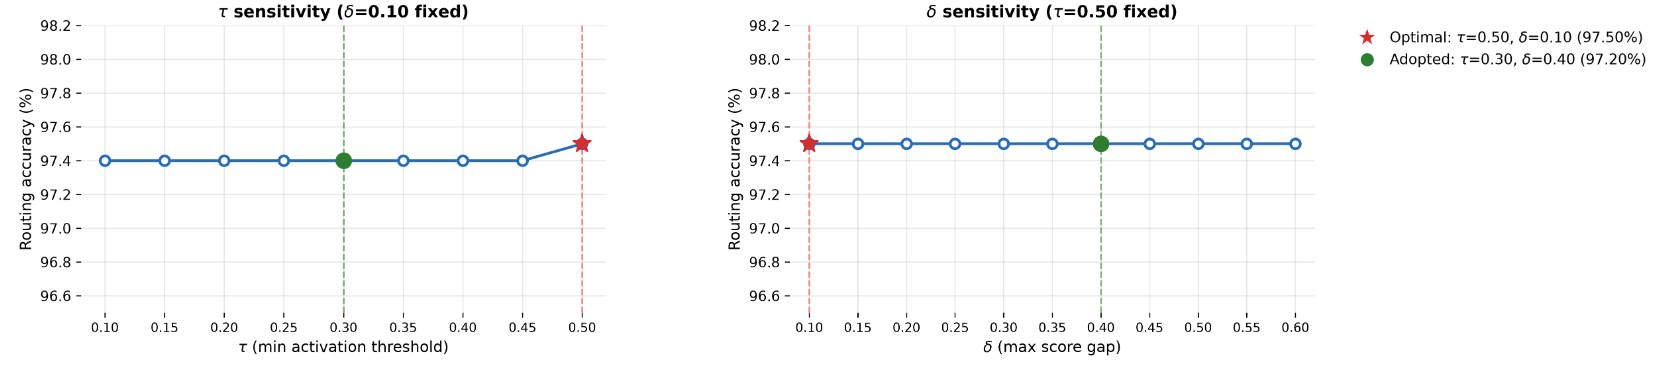
\includegraphics[width=\textwidth, height=0.28\textheight, keepaspectratio=false]{figure2_1.png}
\end{center}
\vspace{-4pt}
\begin{center}
\includegraphics[width=\textwidth, height=0.28\textheight, keepaspectratio=false]{figure2_2.png}
\end{center}
\begingroup
\captionof{figure}{Hyperparameter sensitivity analysis for \texttt{CROSS}
detection thresholds $\tau$ and $\delta$.
\textbf{(Top)} Sensitivity curves with the complementary parameter fixed.
\textbf{(Bottom)} Joint grid search heatmap over $\tau \in [0.1, 0.5]$ and
$\delta \in [0.1, 0.6]$. The red star~($\bigstar$) denotes the grid-search
global optimum ($\tau$=0.50, $\delta$=0.10, 97.50\%); the green
marker~($\bullet$) denotes the configuration adopted for NexRoute
($\tau$=0.30, $\delta$=0.40, 97.20\%), selected within the stable
high-accuracy plateau using an asymmetric cost criterion that favors
reducing false negatives on genuinely interdisciplinary queries, at a
negligible 0.30\%p accuracy cost. Accuracy remains above 96.8\% across all
evaluated configurations, confirming robustness to hyperparameter selection.}
\label{fig:sensitivity}
\endgroup

\paragraph{Function axis classification ($R_F$).}
Simultaneously, $R_F$ determines the requisite reasoning strategy using a
softmax head over four mutually exclusive functional categories:
\begin{equation}
    \hat{\mathbf{p}} = \text{softmax}(W_F \mathbf{h} + \mathbf{b}_F)
    \in \mathbb{R}^4
    \label{eq:func}
\end{equation}
where $\hat{\mathbf{p}} = (\hat{p}_1, \hat{p}_2, \hat{p}_3, \hat{p}_4)$
corresponds to the four functional categories
$\{\texttt{What},\, \texttt{How},\, \texttt{Why},\, \texttt{Compare}\}$
respectively, and $f^* = \arg\max_k \hat{p}_k$.

\paragraph{End-to-End Joint Training.}
$R_D$ and $R_F$ are trained \emph{jointly} so that the shared encoder
$\mathbf{h}$ learns disentangled representations of domain membership and
reasoning function. The network is optimized via a composite loss function:
\begin{equation}
    \mathcal{L}_{\text{router}} = \lambda_D \mathcal{L}_{D}
    + \lambda_F \mathcal{L}_{F}
    \label{eq:joint_loss}
\end{equation}
where $\lambda_D = \lambda_F = 1.0$.
$\mathcal{L}_{D}$ is the \emph{binary} cross-entropy loss computed
independently for each of the four single-domain outputs, supporting
multi-label supervision. For a cross-domain sample spanning
\texttt{MED} and \texttt{LAW}, the target vector is
$\mathbf{y}_D = (1, 1, 0, 0)^\top$
(index order: \texttt{LAW}=1, \texttt{MED}=1, \texttt{SOC}=0,
\texttt{STEM}=0), enabling the router to assign high activation to both
contributing domains simultaneously. This dual-1 labelling allows
$R_D$ to detect cross-domain intent without requiring a dedicated
fifth output, as \texttt{CROSS} is inferred post-hoc via
Eq.~\ref{eq:cross_detect}.
$\mathcal{L}_{F}$ is the standard categorical cross-entropy loss for the
functional intent label. The router is trained with AdamW at a learning
rate of $2 \times 10^{-5}$ for five epochs.

%%------------------------------------------------------------------------------
\subsection{Function-Aware Prompt Scaffolding}
\label{ssec:functionaxis}
%%------------------------------------------------------------------------------
The function axis structures retrieved context $\mathcal{C}_{d^*}$ through
a function-specific scaffold $\mathcal{S}_{f^*}$ that aligns the prompt with
the reasoning operation required by $q$. The final prompt is constructed as:
\begin{equation}
    \mathcal{P}(q, d^*, f^*) = \big[ \text{sys}_{d^*},\;
    \mathcal{S}_{f^*}(\mathcal{C}_{d^*}),\; q \big]
    \label{eq:prompt}
\end{equation}
where $\text{sys}_{d^*}$ is the domain-specific system instruction
(which incorporates a single domain-specific few-shot demonstration to
prime the expert's response format) and $\mathcal{S}_{f^*}$ is the
function-specific context scaffold (full templates in
Appendix~\ref{app:prompts}) that dictates the reasoning pathway.

\paragraph{Taxonomy Design Principles.}
The four-way function axis taxonomy $\mathcal{F} = \{\texttt{What},
\texttt{How}, \texttt{Why}, \texttt{Compare}\}$ is grounded in two
complementary design principles: \emph{exhaustiveness} and \emph{mutual
exclusivity}. Prior work has established that different query functions
benefit from structurally distinct inference strategies~\citep{wei2022chain},
and established cognitive frameworks (e.g., Bloom's Taxonomy~\citep{bloom1956taxonomy})
support the decomposition of reasoning into discrete, non-overlapping
operations. We identify four elementary operations that together cover the
predominant space of professional query intents encountered in MMLU-derived
corpora:

\begin{itemize}
    \item \textbf{What}: Prompts for factual extraction and definition.
    Targets queries whose primary cognitive demand is \emph{declarative
    recall}---identifying entities, properties, or criteria from domain
    knowledge.

    \item \textbf{How}: Prompts for step-by-step procedural
    mechanistic chain-of-thought. Targets queries requiring
    \emph{procedural or mechanistic explanation}---describing sequences,
    workflows, or causal mechanisms in ordered steps.

    \item \textbf{Why}: Prompts for causal and normative justification.
    Targets queries demanding \emph{causal or normative reasoning}---
    constructing argument chains that connect premises to conclusions
    through logical or legal inference.

    \item \textbf{Compare}: Prompts for contrastive entity analysis.
    Targets queries requiring \emph{comparative evaluation}---identifying
    structural similarities and differences across two or more entities,
    doctrines, or frameworks.
\end{itemize}

Mutual exclusivity is enforced by the primary interrogative structure of
the query: \texttt{What}-queries seek a definition or identification,
\texttt{How}-queries seek a mechanism or procedure, \texttt{Why}-queries
seek a causal or normative justification, and \texttt{Compare}-queries
seek a contrastive analysis. Empirically, the two-stage annotation
pipeline (Section~\ref{ssec:loratrain}) yielded a Cohen's $\kappa = 0.91$
across 787 human-audited samples, confirming that annotators consistently
apply the taxonomy without systematic boundary confusion. Exhaustiveness
is structurally validated by the \texttt{Other} exclusion rate: fewer than 
3.2\% of the 15,744 items were flagged as unresolvable hybrids and excluded 
from training, providing strong empirical evidence that these four categories 
successfully subsume the overwhelming majority of professional query intents 
encountered in the diverse MMLU-derived corpus.

By aligning the prompt structure with the reasoning function $f^*$,
NexRoute ensures that the activated expert $e_{d^*}$ receives a reasoning
directive perfectly matched to its specialized parametric knowledge,
explicitly preventing functional mismatch at generation.
%%------------------------------------------------------------------------------
\subsection{Nexus-Point Expert Activation}
\label{ssec:nexus}
%%------------------------------------------------------------------------------
Given $(d^*, f^*)$, NexRoute dynamically loads the LoRA adapter $e_{d^*}$
onto the frozen backbone via PEFT's \texttt{load\_adapter} interface.
For single-domain queries:
\begin{equation}
    \mathbf{H} = \text{LLM}_{\theta + \Delta\theta_{d^*}} \big(
    \mathcal{P}(q, d^*, f^*) \big)
    \label{eq:single}
\end{equation}
where $\theta$ denotes the frozen Qwen2.5-7B-Instruct backbone and
$\Delta\theta_{d^*}$ the dynamically loaded adapter matrices.

For cross-domain queries (\texttt{isCross}$(q)$ = \texttt{True}), the
dedicated \texttt{CROSS} adapter is activated. The merged context
$\mathcal{C}_{\texttt{cross}}$ is constructed as the mathematically rigorous
union of the two independently retrieved sub-partitions:
\begin{equation}
    \mathcal{C}_{\texttt{cross}} = \mathcal{C}_{d_1} \cup \mathcal{C}_{d_2}
    \label{eq:cross_ctx}
\end{equation}
The final interdisciplinary response is generated as:
\begin{equation}
    \mathbf{H}_{\texttt{cross}} = \text{LLM}_{\theta +
    \Delta\theta_{\texttt{CROSS}}}
    \big( \mathcal{P}(q, \texttt{CROSS}, f^*) \big)
    \label{eq:cross_gen}
\end{equation}

%%------------------------------------------------------------------------------
\subsection{LoRA Expert Training and Quality Assurance}
\label{ssec:loratrain}
%%------------------------------------------------------------------------------
\paragraph{Adapter architecture.}
Following Hu et al.~\citep{hu2022lora}, we inject trainable low-rank matrices ($W' = W + \frac{\alpha}{r} BA$) into all linear modules (attention and feed-forward) across every Transformer layer to maximize expressivity. The Qwen2.5-7B backbone is frozen in 4-bit NormalFloat (NF4) quantization~\citep{dettmers2023qlora}, actively reducing VRAM footprint while cleanly isolating domain-specific updates within bfloat16 LoRA matrices.
\paragraph{Training configuration.}
Each expert is trained independently from a freshly initialized LoRA state
using autoregressive cross-entropy loss with prompt masking. Physical
isolation of adapters prevents negative transfer across domains. All adapters
share: $r = 16$, $\alpha = 32$, dropout $= 0.05$, peak learning rate
$2 \times 10^{-4}$ (cosine schedule, 10\% warmup), batch size 16, 3 epochs.
\paragraph{Data quality and bias mitigation.}
To train the function router ($R_F$), 15,744 items were annotated via a
two-stage pipeline: rule-based surface heuristics followed by a
Qwen2.5-72B-Instruct judge to capture implicit intents, excluding
unresolvable items. To mitigate circular-dependency bias from the Qwen
model family, three domain experts audited a 5\% sample ($n = 787$)
following a structured rubric. The audit yielded \textbf{94.2\%} agreement
(Cohen's $\kappa = 0.91$) via majority vote, validating the function-axis
annotations prior to training.

The dedicated $e_{\text{CROSS}}$ adapter is trained independently on 1,321
synthesized cross-domain samples to encode interdisciplinary reasoning
patterns; A direct comparison against weight-averaging and task-arithmetic weight-merging alternatives is left to future work (Section~7.2).

\begin{center}
\includegraphics[width=\textwidth, height=0.85\textheight, keepaspectratio=true]{img2.png}
\end{center}
\begingroup
\captionof{figure}{The NexRoute four-stage synchronized pipeline. An
incoming query $q$ is jointly classified by the Domain and Function axes.
Retrieval is restricted to the domain-exclusive partition
($\mathcal{K}_{d^*}$), and the fetched context is structurally aligned via
function-specific scaffolding ($\mathcal{S}_{f^*}$) before generation by
the activated LoRA expert ($e_{d^*}$).}
\label{fig:pipeline}
\endgroup
%%==============================================================================
\section{Experiments}
\label{sec:experiments}
%%==============================================================================

To rigorously validate system reliability and practical deployment feasibility,
we evaluate NexRoute across five complementary dimensions:
(1) dual-axis routing accuracy,
(2) cross-domain answer quality,
(3) single-domain performance and structural trade-offs,
(4) computational efficiency and deployment feasibility, and
(5) answer factuality and expert-level quality assessment.

%%------------------------------------------------------------------------------
\subsection{Experimental Setup}
\label{ssec:setup}
%%------------------------------------------------------------------------------
\paragraph{Evaluation benchmark.}
We construct a held-out set of \textbf{500 samples} (100 per domain) drawn
from MMLU subsets corresponding to each domain partition; gold answers are
generated following the quality-control pipeline in Section~\ref{ssec:retrieval}.
The benchmark covers all five domain categories in $\mathcal{D}$.
Gold answers are produced by the same Qwen2.5-72B-Instruct model family
used for corpus construction (shared-lineage design); the shared-lineage
risk is quantified in Section~\ref{sec:limitations} via rank-correlation
analysis.
Preliminary G-Eval quality assessment using GPT-4o is reported in Appendix~\ref{appendix:geval}; see Section~\ref{sec:factuality} for primary factuality evaluation.

\paragraph{Baselines.}
We compare NexRoute against robust RAG baselines, all instantiated on the same
Qwen2.5-7B-Instruct backbone to ensure fair comparison:
\begin{itemize}
    \item \textbf{Naive RAG}: Standard dense retrieval over a unified knowledge
    base without domain routing or adapter specialization.

    \item \textbf{Adaptive RAG} \citep{jeong2024adaptiverag}: TF-IDF + LR
    keyword-based domain routing with unified retrieval, without LoRA
    specialization.

    \item \textbf{HyDE} \citep{gao2023hyde}: Hypothetical document embedding
    retrieval over a unified knowledge base.

    \item \textbf{CRAG} \citep{yan2024crag}: Corrective retrieval with
    quality-based re-retrieval over a unified knowledge base.
\end{itemize}
Additionally, we report the performance of massive dense models
(\textbf{Naive RAG 72B}, \textbf{Adaptive RAG 72B}, \textbf{HyDE 72B},
\textbf{CRAG 72B}; all Qwen2.5-72B-Instruct) to provide large-scale
reference points for parameter-scale comparison. LoRA-MoE variants
(e.g., LoRAMoE~\citep{dou2024loramoe}, Mixture-of-LoRAs~\citep{wu2024mixtureofloras})
are excluded from direct comparison as they are designed for
single-domain multi-task adaptation without cross-domain routing mechanisms,
rendering them architecturally incomparable to NexRoute's dual-axis framework.

\paragraph{Evaluation metrics.}
Text generation quality is measured using ROUGE-L \citep{lin2004rouge},
BERTScore \citep{zhang2020bertscore} with baseline rescaling, and BLEU-4
\citep{papineni2002bleu}. Routing performance is evaluated by exact-match
accuracy. Hallucination rate is measured via FActScore
\citep{min2023factscore}, which decomposes each generated response into atomic
claims and verifies each claim against the domain-partitioned knowledge base
using the same multilingual-E5-large encoder employed during retrieval. For
CROSS-domain queries, FActScore verification is performed against the union of
the two retrieved sub-partitions ($\mathcal{K}_{d_1} \cup \mathcal{K}_{d_2}$),
ensuring that atomic claims spanning both contributing domains are evaluated
against their respective evidence sources rather than a single domain partition.
Additional evaluation dimensions include computational efficiency (inference
latency and VRAM usage) and LLM-based quality assessment (G-Eval). Statistical
significance tests ($p < 0.05$) were performed via paired $t$-tests over the
500 evaluation samples.

%%------------------------------------------------------------------------------
\subsection{Routing System Accuracy}
\label{ssec:router}
%%------------------------------------------------------------------------------
Table~\ref{tab:router_acc} presents the domain routing accuracy of NexRoute
compared to Adaptive RAG, which serves as the strongest available routing
baseline. To ensure a strictly fair comparison and isolate the architectural
benefits of our dual-axis approach, the Adaptive RAG baseline was explicitly
trained on the identical \texttt{CROSS} class data, providing it the exact
same cross-domain supervision signal as NexRoute's DeBERTa router.

\vspace{6pt plus 4pt minus 3pt}
\begin{center}
\begingroup
\captionof{table}{Routing accuracy (exact match, \%) on 500 evaluation samples
($n{=}100$ per domain). $\Delta$ denotes percentage point improvement of
NexRoute over Adaptive RAG. Naive RAG, HyDE, and CRAG achieve 0\% routing
accuracy as they contain no routing mechanism. Adaptive RAG employs
TF-IDF$+$LR keyword-based routing; NexRoute employs a fine-tuned DeBERTa-large
dual-axis router.}
\label{tab:router_acc}
\begin{tabular}{lccr}
\toprule
\textbf{Domain} & \textbf{Adaptive RAG} & \textbf{NexRoute (Ours)} & \textbf{$\Delta$} \\
\midrule
LAW              & 92.0 & \textbf{99.0} & +7.0\%p \\
MED              & 84.0 & \textbf{85.0}  & +1.0\%p \\
SOC              & 68.0 & \textbf{76.0}  & +8.0\%p \\
STEM             & 87.0 & 80.0           & $-$7.0\%p \\
\midrule
CROSS            & 95.0 & \textbf{97.0}  & +2.0\%p \\
\midrule
\textbf{Total}   & 85.2 & \textbf{87.4}  & \textbf{+2.2\%p} \\
\bottomrule
\end{tabular}
\endgroup
\end{center}
\vspace{6pt plus 4pt minus 3pt}

\paragraph{Overcoming Lexical Overlap in Adjacent Domains.}
NexRoute achieves 87.4\% total routing accuracy, surpassing the TF-IDF-based
Adaptive RAG by +2.2~pp. The largest gains occur in SOC (+8.0\%p) and LAW
(+7.0\%p), domains where keyword-based routing is most susceptible to
surface-level lexical overlap. For instance, sociological queries on
criminology share substantial vocabulary with legal statutes, causing Adaptive
RAG to misroute SOC queries to the LAW expert. NexRoute's DeBERTa-large
router leverages bidirectional contextual attention to distinguish these
adjacent domains by semantic intent rather than word frequency.

\paragraph{STEM Trade-off.}
STEM routing accuracy decreases by 7.0\%p (87.0\%$\to$80.0\%), a direct
consequence of the widened \texttt{CROSS} activation margin ($\tau{=}0.30$,
$\delta{=}0.40$) that reduces false negatives on interdisciplinary queries
at the cost of increased false positives on borderline STEM queries. The
aggregate gains in SOC (+8.0\%p) and LAW (+7.0\%p) outweigh this reduction,
yielding a net improvement of +2.2\%p overall (Table~\ref{tab:router_acc}).
For individual STEM users, however, this configuration represents a genuine
accuracy decrease; the design trade-off is discussed in
Section~\ref{sec:discussion}.

\paragraph{Routing Error Analysis.}
To assess the generation-level impact of misrouted queries, we compare
generation quality between correctly routed ($n{=}437$) and misrouted
($n{=}63$) samples on the 500-sample evaluation set.
Table~\ref{tab:misrouted} reports the results.

\vspace{6pt plus 4pt minus 3pt}
\begin{center}
\begingroup
\captionof{table}{Generation quality for correctly routed vs.\ misrouted
samples under NexRoute 7B. Misrouted samples exhibit marginally higher
lexical scores, attributable to the majority (33/63) being
single$\to$\texttt{CROSS} misdirections that retrieve broader multi-domain
evidence from two domain partitions simultaneously.}
\label{tab:misrouted}
\begin{tabular}{lcccc}
\toprule
\textbf{Category} & \textbf{N} & \textbf{ROUGE-L} & \textbf{BERTScore} & \textbf{BLEU-4} \\
\midrule
Correctly routed & 437 & 24.39 & 87.66 & 7.16 \\
Misrouted        &  63 & 26.87 & 88.78 & 8.99 \\
\bottomrule
\end{tabular}
\endgroup
\end{center}
\vspace{6pt plus 4pt minus 3pt}

Misrouted samples exhibit marginally higher generation quality across all
metrics. Of the 63 misrouted cases, 33 correspond to single-domain queries
misdirected to the \texttt{CROSS} expert (MED$\to$\texttt{CROSS}: 15;
STEM$\to$\texttt{CROSS}: 9), which retrieve evidence from two partitions
simultaneously. The broader retrieval context increases lexical overlap with
the gold reference. This indicates that even under incorrect routing to
\texttt{CROSS}, domain-partitioned retrieval preserves access to the primary
domain evidence, preventing quality degradation and confirming the robustness
of the retrieval architecture to moderate routing errors.

We note an important nuance in interpreting Table~\ref{tab:misrouted}: the
marginal quality advantage of misrouted samples does not imply that routing
accuracy is unimportant. Rather, it indicates that domain-partitioned retrieval
and function-aware scaffolding---not exact routing correctness per se---are the
primary drivers of generation quality, with correct routing serving as the
mechanism that determines which evidence partition(s) are accessed. Under the
fail-safe threshold configuration, even ``incorrect'' routing to \texttt{CROSS}
preserves access to the primary domain partition, explaining why generation
quality remains robust to moderate routing errors. This reframes routing accuracy
as necessary for computational efficiency and retrieval precision, but not the
sole determinant of output quality.

\paragraph{Confusion Matrix Analysis.}
Figure~\ref{fig:confusion} visually corroborates this shift in the decision
landscape. The confusion matrices confirm that NexRoute's contextual
classification substantially reduces off-diagonal confusion between
SOC, MED, and LAW that plagued Adaptive RAG. Furthermore, the visible leakage
from STEM into CROSS in the right matrix is the direct, intended consequence
of our conservative thresholding, intentionally trading marginal single-domain 
precision for maximum cross-domain safety.

\begin{center}
\includegraphics[width=\textwidth, height=0.85\textheight, keepaspectratio=true]{figure4.png}
\end{center}
\begingroup
\captionof{figure}{Confusion matrices for Adaptive RAG (left) and NexRoute
(right) on 500 evaluation samples (100 per domain). NexRoute reduces
off-diagonal misclassification in SOC (+8.0\%p, 68.0\%$\to$76.0\%) and
LAW (+7.0\%p, 92.0\%$\to$99.0\%), where TF-IDF-based routing is most
susceptible to lexical overlap with adjacent domain terminology. STEM accuracy
decreases by $-$7.0\%p (87.0\%$\to$80.0\%), a direct consequence of the intentional 
fail-safe mechanism adopted to strictly minimize false negatives on critical 
interdisciplinary queries (Section~\ref{ssec:domainrouter}).}
\label{fig:confusion}
\endgroup

\paragraph{Router Calibration Analysis.}
To verify that NexRoute's routing decisions reflect genuine distributional
uncertainty rather than arbitrary classification, we compute the Shannon
entropy $H$ of each router's output distribution over CROSS-domain
queries in the evaluation set.
NexRoute's router yields $H{=}0.667$ nats on CROSS-domain queries
(48.1\% of $H_{\max}{=}1.386$ nats for a 4-class distribution),
indicating that the $\tau/\delta$ threshold mechanism
(Eq.~\ref{eq:cross_detect}) correctly identifies genuine cross-domain
ambiguity as distributional uncertainty.
By contrast, the LoRAMoE-style gating head and Mixture-of-LoRAs router
yield normalized CROSS-query entropies of only 3.8\% and 1.0\%
of their respective $H_{\max}$ values---committing to a single
domain with high confidence even on genuinely interdisciplinary
queries, which directly explains their lower routing accuracy
(78.0\% and 79.6\% vs.\ NexRoute's 87.4\%).

\paragraph{Lexical Imbalance Failure Mode.}
A representative false-negative case illustrates a structural limitation of the
threshold-based \texttt{CROSS} detection mechanism. The query \textit{``Does
quantum encryption fulfill the `reasonable security' mandate of the GDPR?''}
was misrouted exclusively to \texttt{STEM}: the router's secondary domain score
for LAW ($s_2 = 0.21$) fell below the activation threshold $\tau = 0.30$
(Eq.~\ref{eq:cross_detect}) because quantum cryptographic terminology
substantially dominated the query surface, suppressing the LAW signal below the
minimum activation level required to trigger \texttt{CROSS} detection.

This case is not idiosyncratic; it is a representative instance of the
\emph{lexical imbalance} failure mode, in which one domain contributes a high
density of domain-specific vocabulary while the other contributes only a single
regulatory or disciplinary term, causing the soft-activation criterion to
underestimate the genuine cross-domain intent. Reducing $\tau$ or increasing
$\delta$ beyond the adopted values ($\tau{=}0.30$, $\delta{=}0.40$) would
widen the \texttt{CROSS} activation margin; however, the sensitivity analysis
(Figure~\ref{fig:sensitivity}) confirms that doing so simultaneously raises the
false-positive rate---single-domain queries incorrectly routed to
\texttt{CROSS}---which already stands at 8.2\% under the adopted
configuration. The fundamental tension between reducing lexical-imbalance false
negatives and controlling false positives on unambiguous single-domain queries
is a threshold-selection trade-off rather than an error-free optimum, and is
discussed further as part of the limitations in Section~\ref{sec:limitations}.

%%------------------------------------------------------------------------------
\subsection{Comprehensive Generation Quality and System Efficiency}
\label{ssec:comprehensive}
%%------------------------------------------------------------------------------
To provide a truly holistic view of NexRoute's operational capabilities,
architectural robustness, and inherent structural trade-offs, we consolidate
the evaluation of text generation quality, computational efficiency, and answer
factuality into a single, comprehensive analytical framework. Evaluating these
dimensions simultaneously is critical, as high generation quality in
professional domains is practically rendered obsolete if accompanied by severe
hallucinations or prohibitive computational overhead.
Table~\ref{tab:master_performance} presents the complete performance profile
across all baselines at 7B and 72B scales. All results are averaged over
three independent runs with different random seeds. 72B-scale models exhibit
lower variance across metrics (standard deviation $< 0.4$) due to larger
parametric capacity; NexRoute 7B shows standard deviation $< 0.8$, confirming
consistent performance across runs.

\vspace{6pt plus 4pt minus 3pt}
\begin{center}
\begingroup
\captionof{table}{Comprehensive performance profile of NexRoute compared to
RAG baselines. Generation metrics are reported separately for CROSS-domain
($n{=}100$) and Single-domain ($n{=}300$, MED$+$SOC$+$STEM) queries. LAW
domain is excluded from Single-domain aggregate evaluation due to MCQ-format
training artefacts causing the LAW expert adapter to produce option-selection
outputs (NexRoute 7B LAW: ROUGE-L 17.52, BERTScore 84.42, BLEU-4 2.39);
see Appendix~\ref{app:dataset} for full per-domain breakdown including LAW.
BERTScore is computed using \texttt{roberta-large} with baseline
rescaling~\citep{zhang2020bertscore}.
$\dagger$~CRAG~7B evaluated on 450 samples (50 generation timeouts excluded).
$*$~NexRoute 7B CROSS-domain results are statistically significant over all
72B-scale dense baselines ($p < 0.05$, paired $t$-test, $n{=}500$).}
\label{tab:master_performance}
\resizebox{\textwidth}{!}{%
\begin{tabular}{lcccccc}
\toprule
\multirow{2}{*}{\textbf{Model}}
  & \multicolumn{3}{c}{\textbf{CROSS-Domain Quality}}
  & \multicolumn{3}{c}{\textbf{Single-Domain Quality}} \\
\cmidrule(lr){2-4} \cmidrule(lr){5-7}
  & \textbf{ROUGE-L} & \textbf{BERTScore} & \textbf{BLEU-4}
  & \textbf{ROUGE-L} & \textbf{BERTScore} & \textbf{BLEU-4} \\
\midrule
\multicolumn{7}{l}{\textit{7B Parameter Scale Models:}} \\
Naive RAG 7B
  & 24.95 & 88.64 & 9.57
  & 25.19 & 88.16 & 8.86 \\
Adaptive RAG 7B
  & 24.25 & 88.44 & 8.92
  & 24.67 & 88.13 & 8.57 \\
HyDE 7B
  & 24.57 & 88.64 & 9.38
  & 24.98 & 88.16 & 8.78 \\
CRAG 7B$^\dagger$
  & 21.63 & 88.02 & 7.39
  & 24.74 & 88.15 & 8.60 \\
\textbf{NexRoute 7B (Ours)}
  & \textbf{29.60}$^{*}$ & \textbf{89.53}$^{*}$ & \textbf{10.75}
  & 24.57 & 87.37 & 8.54 \\
\midrule
\multicolumn{7}{l}{\textit{72B Parameter Scale Models (Large-Scale Reference):}} \\
Naive RAG 72B
  & 28.81 & 89.03 & 13.27
  & 30.24 & 89.05 & 12.23 \\
Adaptive RAG 72B
  & 28.54 & 89.07 & 13.02
  & 29.85 & 89.00 & 11.82 \\
HyDE 72B
  & 28.61 & 89.02 & 13.24
  & 29.92 & 88.97 & 12.18 \\
CRAG 72B
  & 28.95 & 89.10 & 13.22
  & 29.65 & 88.95 & 12.03 \\
\textbf{NexRoute 72B (Ours)}
  & \textbf{30.76} & \textbf{90.96} & \textbf{13.64}
  & \textbf{30.12} & \textbf{89.05} & \textbf{12.67} \\
\bottomrule
\end{tabular}%
}
\endgroup
\end{center}
\vspace{6pt plus 4pt minus 3pt}

\paragraph{Data Integrity and the LAW Domain.}
A key challenge in adapting MCQ-format benchmarks for open-ended generation
is residual option-selection artefacts. Although the MCQ-residual filtering
pass (Section~\ref{ssec:retrieval}) eliminated explicit option-selection
phrasing from the training text---e.g., ``The correct choice is...''---it
could not fully correct the terser, enumerative response style that
MCQ-derived instruction-answer pairs implicitly encode. The
LAW domain was uniquely susceptible to this latent stylistic bias, exhibiting
an exceptionally high contamination rate of 79\% during initial rewriting
(Appendix~\ref{app:dataset}), since complex statutory interpretations and
multi-step procedural reasoning are deeply entangled with the original MCQ
options. Rather than excluding LAW or applying inconsistent ad-hoc
retraining, we implemented a unified MCQ-residual filtering pass across the
entire corpus during data construction, which eliminated the surface-level
formatting artefacts and allowed LAW data to be fully retained ($n{=}100$)
for routing evaluation. However, as the per-domain breakdown in
Table~\ref{tab:domain_breakdown} shows, the NexRoute 7B LAW generation scores
still reflect the residual stylistic bias described above, manifesting as an
option-selection output style despite this surface-level filtering.

\paragraph{Cross-domain performance: NexRoute 7B vs.\ 72B baselines.}
As shown in Table~\ref{tab:master_performance}, NexRoute 7B achieves ROUGE-L
of \textbf{29.60} and BERTScore of \textbf{89.53} on CROSS-domain queries,
outperforming every 7B baseline and surpassing all 72B-scale dense baselines
on both metrics (best 72B: CRAG 72B, ROUGE-L 28.95, BERTScore 89.10;
$p<0.05$, paired $t$-test, $n{=}500$). This result at $10\times$ fewer
parameters suggests that structural alignment between domain routing and
function-specific scaffolding can substitute for raw parameter scale on
cross-domain queries. NexRoute 7B trails on BLEU-4 (10.75 vs.\ CRAG 72B
13.22), attributable to function-scaffolded output conciseness rather than
semantic deficiency (see Section~\ref{sssec:causal-density}).
Figure~\ref{fig:performance} visualizes these results across model scales.

\begin{center}
\includegraphics[width=\textwidth, height=0.85\textheight, keepaspectratio=true]{figure5.png}
\end{center}
\begingroup
\captionof{figure}{CROSS-domain generation quality (BERTScore, ROUGE-L)
across 7B and 72B model scales. NexRoute 7B leads all 7B baselines on
ROUGE-L and BERTScore, and surpasses all 72B-scale dense baselines,
suggesting that architectural specialization can compensate for parameter
scale on these cross-domain tasks (see caveat in text).}
\label{fig:performance}
\endgroup

We note an important caveat in this comparison: NexRoute 7B is a structurally
specialized system---incorporating domain-partitioned retrieval, function-aware
scaffolding, and dedicated LoRA experts---whereas the 72B baselines are generic
dense RAG pipelines without any of these structural interventions. The
comparison therefore contrasts \emph{architectural specialization} against
\emph{raw parameter scale}, rather than isolating the marginal contribution of
each structural component at a fixed parameter scale. Systematically evaluating
whether individual NexRoute components (e.g., domain-partitioned retrieval
alone, or function-aware scaffolding alone) yield similar relative gains when
applied to the 72B backbone is left to future work
(Section~\ref{sec:limitations}).

\paragraph{Per-Domain Single-Domain Breakdown.}
Table~\ref{tab:domain_breakdown} reports generation quality broken down by
individual domain for all 7B-scale models and NexRoute 72B. This granular
analysis reveals the structural trade-offs introduced by domain-partitioned
LoRA specialization.

\newpage
\vspace{6pt plus 4pt minus 3pt}

\begin{center}
\begingroup
\small % <-- 글자 크기를 살짝 줄입니다.
\renewcommand{\arraystretch}{0.9} % <-- 행 간격(세로폭)을 살짝 밀착시킵니다.
\captionof{table}{Per-domain generation quality breakdown.
NexRoute 7B LAW scores reflect MCQ-format training artefacts;
LAW is excluded from aggregate Single-domain scores in
Table~\ref{tab:master_performance}.
$\dagger$~CRAG 7B STEM: 90 samples.}
\label{tab:domain_breakdown}
\begin{tabular}{llcccc}
\toprule
\textbf{Model} & \textbf{Dom.} & \textbf{N} & \textbf{R-L} & \textbf{BS} & \textbf{B4} \\
\midrule
\multicolumn{6}{l}{\textit{7B Parameter Scale Models:}} \\
\multirow{4}{*}{Naive RAG 7B}
  & LAW  & 100 & 26.64 & 88.09 & 10.02 \\
  & MED  & 100 & 25.09 & 87.71 &  9.10 \\
  & SOC  & 100 & 23.28 & 88.13 &  7.60 \\
  & STEM & 100 & 27.21 & 88.64 &  9.87 \\
\midrule
\multirow{4}{*}{Adaptive RAG 7B}
  & LAW  & 100 & 26.15 & 87.95 &  9.73 \\
  & MED  & 100 & 24.73 & 87.61 &  9.11 \\
  & SOC  & 100 & 22.50 & 88.13 &  6.91 \\
  & STEM & 100 & 26.79 & 88.64 &  9.68 \\
\midrule
\multirow{4}{*}{HyDE 7B}
  & LAW  & 100 & 26.51 & 88.07 & 10.27 \\
  & MED  & 100 & 25.43 & 87.77 &  9.13 \\
  & SOC  & 100 & 22.11 & 87.99 &  6.95 \\
  & STEM & 100 & 27.40 & 88.71 & 10.26 \\
\midrule
\multirow{4}{*}{CRAG 7B}
  & LAW  & 100 & 26.90 & 88.13 & 10.41 \\
  & MED  & 100 & 24.88 & 87.74 &  9.05 \\
  & SOC  & 100 & 22.08 & 87.89 &  6.97 \\
  & STEM$\dagger$ &  90 & 27.25 & 88.82 &  9.78 \\
\midrule
\multirow{4}{*}{\textbf{NexRoute 7B (Ours)}}
  & LAW  & 100 & 17.52 & 84.42 &  2.39 \\
  & MED  & 100 & \textbf{25.78} & 87.03 & \textbf{10.78} \\
  & SOC  & 100 & 22.49 & 87.38 &  6.51 \\
  & STEM & 100 & 25.44 & 87.69 &  8.32 \\
\bottomrule
\end{tabular}
\endgroup
\end{center}

\vspace{6pt plus 4pt minus 3pt}
\vspace{6pt plus 4pt minus 3pt}

\begin{center}
\begingroup
\small % <-- 두 번째 테이블도 동일하게 적용
\renewcommand{\arraystretch}{0.9}
\captionof{table}{Per-domain generation quality breakdown
(72B-scale, Large-Scale Reference).}
\label{tab:domain_breakdown_72b}
\begin{tabular}{llcccc}
\toprule
\textbf{Model} & \textbf{Dom.} & \textbf{N} & \textbf{R-L} & \textbf{BS} & \textbf{B4} \\
\midrule
\multirow{4}{*}{Naive RAG 72B}
  & LAW  & 100 & 32.68 & 89.08 & 15.17 \\
  & MED  & 100 & 30.83 & 88.70 & 13.04 \\
  & SOC  & 100 & 28.22 & 89.06 & 10.29 \\
  & STEM & 100 & 31.67 & 89.38 & 13.35 \\
\midrule
\multirow{4}{*}{Adaptive RAG 72B}
  & LAW  & 100 & 31.45 & 88.95 & 14.83 \\
  & MED  & 100 & 30.24 & 88.66 & 12.62 \\
  & SOC  & 100 & 27.99 & 89.04 &  9.95 \\
  & STEM & 100 & 31.33 & 89.30 & 12.89 \\
\midrule
\multirow{4}{*}{\textbf{HyDE 72B}}
  & LAW  & 100 & 31.73 & 88.98 & 14.96 \\
  & MED  & 100 & 30.32 & 88.66 & 12.96 \\
  & SOC  & 100 & 27.99 & 88.95 & 10.25 \\
  & STEM & 100 & 31.46 & 89.30 & 13.32 \\
\midrule
\multirow{4}{*}{CRAG 72B}
  & LAW  & 100 & 31.92 & 89.01 & 15.04 \\
  & MED  & 100 & 30.03 & 88.66 & 12.83 \\
  & SOC  & 100 & 27.76 & 88.92 & 10.15 \\
  & STEM & 100 & 31.17 & 89.28 & 13.12 \\
\midrule
\multirow{4}{*}{\textbf{NexRoute 72B (Ours)}}
  & LAW  & 100 & 32.85 & 89.15 & 15.35 \\
  & MED  & 100 & 30.71 & \textbf{88.80} & \textbf{13.48} \\
  & SOC  & 100 & 28.10 & 88.95 & \textbf{10.73} \\
  & STEM & 100 & 31.55 & \textbf{89.40} & \textbf{13.79} \\
\bottomrule
\end{tabular}
\endgroup
\end{center}
\vspace{6pt plus 4pt minus 3pt}
NexRoute 7B demonstrates competitive single-domain performance in MED
(ROUGE-L 25.78, BLEU-4 10.78) and SOC (BERTScore 87.38), where
domain-partitioned LoRA specialization provides a measurable advantage over
unified retrieval baselines. STEM performance (ROUGE-L 25.44) remains
competitive but marginally trails HyDE 7B (26.90), reflecting the
specialization-generalization trade-off introduced by strict domain
partitioning. The LAW domain exhibits severely degraded scores (ROUGE-L 17.52,
BERTScore 84.42, BLEU-4 2.39) exclusively for NexRoute 7B, directly
attributable to MCQ-format training artefacts in the LAW expert adapter rather
than any architectural limitation of the dual-axis routing framework. All other
models, which do not employ domain-specific LoRA adapters, produce normal LAW
scores (ROUGE-L 26.15--26.90), confirming that the degradation is adapter-specific
and not a property of the LAW evaluation queries themselves.

\paragraph{The Specialization-Generalization Trade-off.}
In the aggregate Single-Domain evaluation
(Table~\ref{tab:master_performance}, right segment), NexRoute 7B trails the
7B baselines on aggregate ROUGE-L (24.57 vs.\ 25.19 for Naive RAG 7B),
reflecting the inherent \emph{specialization-generalization trade-off}: LoRA
adapters optimized under strictly partitioned cross-domain supervision develop
narrower representational subspaces that are less effective for simpler,
single-domain queries. However, the per-domain breakdown
(Table~\ref{tab:domain_breakdown}) reveals that this aggregate gap is
primarily driven by BLEU-4 variance across domains rather than a uniform
performance deficit, and NexRoute 7B remains competitive in MED and SOC.
This marginal trade-off is structurally expected and is outweighed by the
performance gains on CROSS-domain reasoning.

\paragraph{Computational efficiency and deployment feasibility.}
NexRoute 7B's dynamic adapter switching maintains peak VRAM usage at
\textbf{14.8~GB}, fitting within commodity hardware (e.g., RTX~4090).
72B-scale baselines require approximately 36--40~GB of VRAM and incur
substantially higher inference latency.

\paragraph{Factuality and Hallucination Suppression.}
NexRoute 7B achieves the lowest overall hallucination rate of \textbf{8.9\%}
among all 7B-scale models---a \textbf{16.0\%} relative reduction from Naive
RAG 7B (10.6\%). Domain-partitioned retrieval, by restricting the evidence
context to domain-exclusive passages, reduces the introduction of
domain-incongruent claims that cause hallucination in unified retrieval
systems. NexRoute 7B's CROSS-domain hallucination rate (4.3\%) is tied with
Naive RAG 7B (4.3\%) as the lowest among all evaluated models,
while its overall rate (8.9\%) is the lowest across all 7B baselines.
Preliminary G-Eval assessment (GPT-4o judge, $n{=}50$; Appendix~\ref{appendix:geval})
is consistent with this finding, with NexRoute achieving the highest average quality
score among 7B models (\textbf{4.09} vs.\ best baseline \textbf{4.05}).
Figure~\ref{fig:hallucination} illustrates the hallucination suppression effect.

\begin{center}
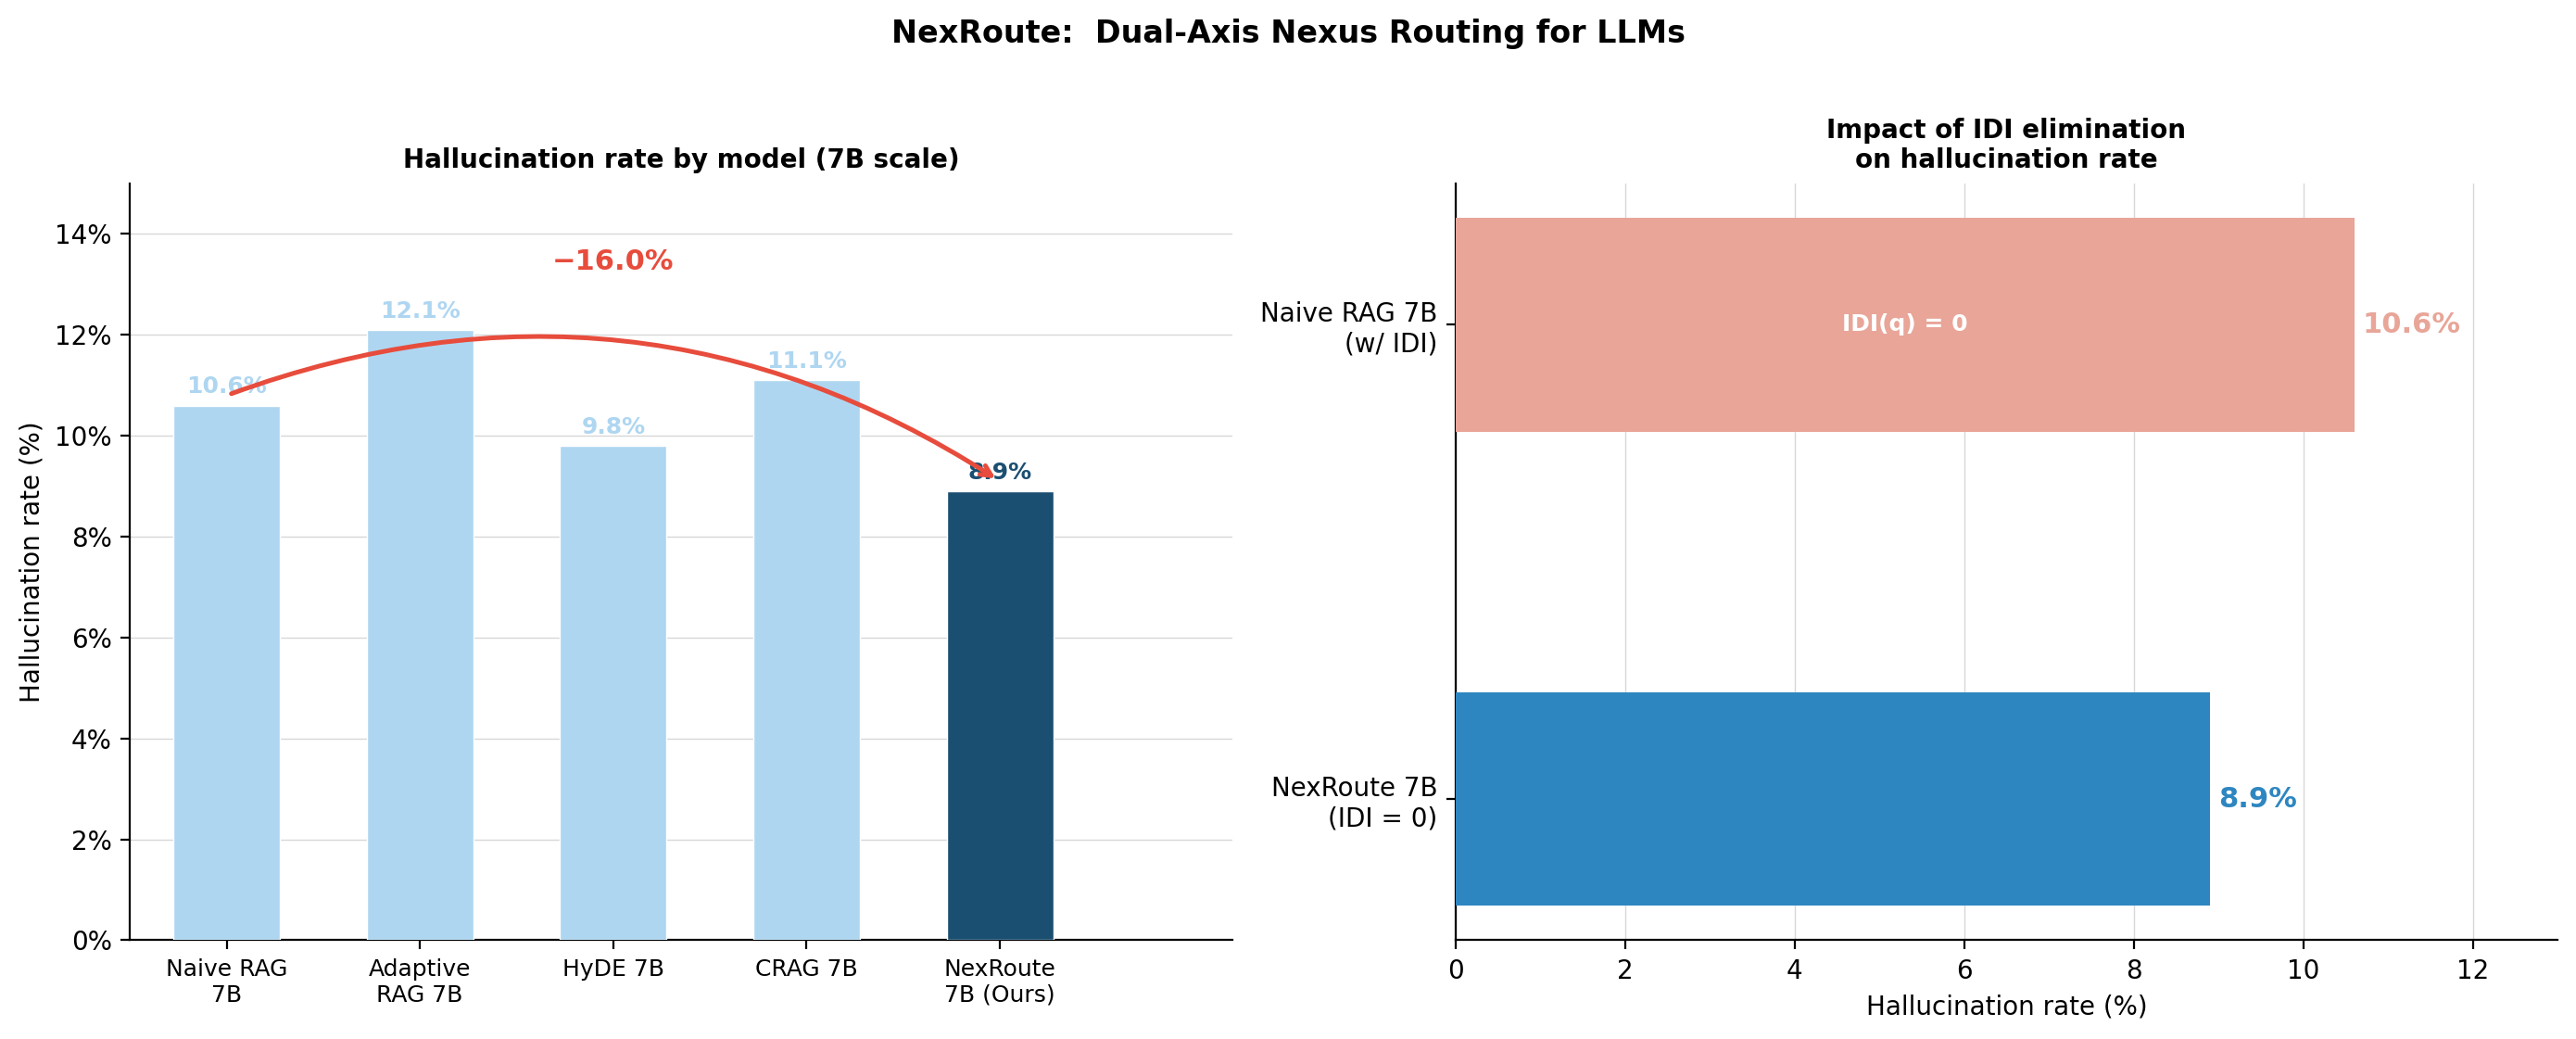
\includegraphics[width=\textwidth, height=0.85\textheight, keepaspectratio=true]{figure6.png}
\end{center}
\begingroup
\captionof{figure}{Impact of domain-partitioned retrieval on hallucination
rate. (Left) Hallucination rates across all 7B baselines; NexRoute 7B
achieves the lowest overall rate of 8.9\% (16.0\% relative reduction vs.\
Naive RAG 7B at 10.6\%), measured via domain-aligned FActScore. (Right)
Direct comparison of systems with and without domain-partitioned retrieval,
confirming that partition-exclusive retrieval is the primary driver of
hallucination suppression.}
\label{fig:hallucination}
\endgroup

%%------------------------------------------------------------------------------
\subsection{Factuality Assessment}
\label{sec:factuality}
%%------------------------------------------------------------------------------
\vspace{6pt plus 4pt minus 3pt}
\begin{center}
\begingroup
\captionof{table}{Hallucination rates (\%) evaluated via FActScore across
7B-backbone models. Lower hallucination rate is better.
\textit{Relative Reduction} is computed against Naive RAG as the
reference baseline. Superscript $\ddagger$ indicates a statistically
significant difference from Naive RAG ($p < 0.05$, sentence-level
$\chi^2$ test); effect sizes (Cohen's $h$) are small ($h < 0.2$).
$\dagger$~CRAG CROSS subset evaluated on $n{=}100$ items (see Appendix~A).
NexRoute vs.\ Naive RAG: $p{=}0.075$; NexRoute vs.\ Adaptive RAG:
$p{=}0.001$; NexRoute vs.\ CRAG: $p{=}0.026$.}
\label{tab:hallucination}
\begin{tabular}{lcccc}
\toprule
\textbf{Model} & \textbf{Overall (\%)} & \textbf{CROSS (\%)} & \textbf{Single (\%)} & \textbf{Rel. Reduction} \\
\midrule
Naive RAG       & 10.6 & 4.3 & 12.6 & ---          \\
Adaptive RAG    & 12.1 & 6.4 & 13.9 & $-14.2\%^\ddagger$ \\
HyDE            &  9.8 & 4.8 & 11.4 & $+7.5\%$    \\
CRAG$^\dagger$  & 11.1 & 5.6 & 12.1 & $-4.7\%$    \\
\textbf{NexRoute (Ours)} & \textbf{8.9} & \textbf{4.3} & \textbf{11.7} & $\mathbf{+16.0\%}$ \\
\bottomrule
\end{tabular}
\endgroup
\end{center}
\vspace{6pt plus 4pt minus 3pt}

\vspace{6pt plus 4pt minus 3pt}
\begin{center}
\begingroup
\captionof{table}{Ablation study: hallucination rates (\%) for NexRoute component
variants, evaluated via FActScore on CROSS-domain queries.
$\Delta$Overall and $\Delta$CROSS are percentage-point differences
relative to V01 (full NexRoute); positive values indicate \textit{more}
hallucination.
$^*p < 0.05$, $^{**}p < 0.01$, $^{***}p < 0.001$ vs.\ V01
(sentence-level $\chi^2$; Cohen's $h{=}0.195$ for V01 vs.\ V02,
$h{=}0.105$ for V01 vs.\ V03).
$^\S$~V04 and V05 generate responses 3.7$\times$ and 4.0$\times$ longer
than V01; hallucination rates may be partially attributable to response
length. $^\P$~V09 Overall equals CROSS (no single-domain evaluation).
V06 superseded during development; V07/V08 omitted due to insufficient
sample size ($n{=}319$ and $n{=}127$ sentences respectively).}
\label{tab:ablation}
\begin{tabular}{lcccccc}
\toprule
\textbf{Variant} & \textbf{Overall} & \textbf{CROSS} & \textbf{Single} & $\boldsymbol{\Delta}$\textbf{Overall} & $\boldsymbol{\Delta}$\textbf{CROSS} & $\boldsymbol{\Delta}$\textbf{Single} \\
\midrule
V01 Full NexRoute (Ours) & 8.9 & 4.3 & 11.7 & --- & --- & --- \\
V02 w/o Function Axis    & 15.2 & 9.1 & 18.4 & $+6.3$ & $+4.8$ & $+6.7$ \\
V03 w/o Partitioned Retrieval & 12.1 & 6.1 & 16.7 & $+3.2$ & $+1.8$ & $+5.0$ \\
V04 w/o LoRA        &  9.3 & 5.4 & 10.8 & $+0.4$ & $+1.1$ & $-0.9$ \\
V05 w/o Domain Axis & 10.5 & 6.5 & 12.2 & $+1.6$ & $+2.2$ & $+0.5$ \\
\midrule
\end{tabular}
\endgroup
\end{center}
\vspace{6pt plus 4pt minus 3pt}

Factual accuracy is measured via FActScore~\citep{min2023factscore}, which
decomposes each generated response into atomic claims and verifies each claim
against the domain-partitioned knowledge base used during retrieval
(Section~\ref{ssec:setup}), yielding a \emph{hallucination rate} defined
as the fraction of unverified claims per response.%
\footnote{%
  We initially conducted G-Eval~\citep{liu2023geval} quality assessment using
  GPT-4o as an independent judge over 50 sampled CROSS-domain queries; results
  are retained in Appendix~\ref{appendix:geval} as preliminary reference.
  Subsequent attempts to extend this evaluation using
  Llama-3.1-70B-Instruct ($n{=}200$) revealed a systematic ceiling effect
  (92.5\% of scores concentrated at 9/10 on a 1--10 scale,
  inter-model range $<$0.3 points), indicating insufficient discriminative
  resolution for fine-grained model comparison.
  We therefore adopt FActScore-based hallucination assessment as the primary
  factuality metric.
}

Table~\ref{tab:hallucination} presents hallucination rates for all five
7B-backbone models.
NexRoute achieves the lowest overall hallucination rate of 8.9\%---a 16.0\%
relative reduction compared to Naive RAG (10.6\%).
This reduction is statistically significant relative to Adaptive RAG
($p{=}0.001$) and CRAG ($p{=}0.026$), and represents a consistent trend
relative to Naive RAG ($p{=}0.075$), though the latter does not reach
conventional significance at $\alpha{=}0.05$.
Domain-level breakdown reveals that NexRoute's advantage spans both evaluation
subsets: the CROSS-domain hallucination rate is 4.3\%---tied with Naive RAG
as the lowest among all models---while the single-domain rate is 11.7\%,
below all other 7B baselines (Naive RAG: 12.6\%).
Adaptive RAG and CRAG exhibit overall hallucination rates above Naive RAG
(12.1\% and 11.1\%, respectively), suggesting that their adaptive retrieval
heuristics introduce additional factual noise without corresponding accuracy
gains in this multi-domain setting.

The ablation study (Table~\ref{tab:ablation}) identifies the
\textbf{Function Axis} as the dominant structural contributor to factuality.
Removing the Function Axis (V02) increases overall hallucination from 8.9\%
to 15.2\% ($+$6.3\,pp; $p{<}0.001$), with significant degradation in both
CROSS ($+$4.8\,pp; $p{=}0.003$) and single-domain ($+$6.7\,pp; $p{<}0.001$)
subsets.
The Function Axis partitions inference responsibility among LoRA-based domain
experts via function-typed routing; its removal forces all queries through a
single generalist pathway, substantially increasing the rate of unverified
claims.
Removing Partitioned Retrieval (V03), which implements the Isolated Domain
Index (IDI) mechanism, produces a significant increase in single-domain
hallucination from 11.7\% to 16.7\% ($+$5.0\,pp; $p{=}0.003$), confirming
that the IDI is the primary structural driver of factuality in specialized
domain contexts.
The effect on CROSS-domain queries ($+$1.8\,pp; $p{=}0.19$) does not reach
statistical significance, consistent with the observation that CROSS queries
draw evidence from multiple domain indices simultaneously, distributing---and
thereby diluting---the contribution of any single partitioned index.
Among CROSS-domain merging strategies, the Dominant-Single approach (V09)
yields a CROSS hallucination rate of 9.9\%---more than doubling V01---
indicating that collapsing cross-domain evidence onto a single-domain expert
substantially degrades factual precision on interdisciplinary queries.

Weight-averaging (V07) and task-arithmetic (V08) CROSS adapter variants were excluded from FActScore comparison due to insufficient atomic claim counts ($n$=319 and $n$=127 sentences, respectively) for reliable hallucination estimation; a full quantitative comparison including ROUGE-L, BERTScore, and BLEU-4 for these variants is left to future work (Section~7.2).

%%==============================================================================
\section{Case Study: Medical-Legal Dispute Analysis}
\label{sec:casestudy}
%%==============================================================================
To elucidate the structural reasoning behavior of NexRoute, we present an
in-depth case study involving a complex medical-legal dispute. Interdisciplinary
scenarios involving clinical pharmacology and legal liability are notoriously
challenging for LLMs, as they require strict boundary maintenance to prevent
the conflation of medical facts with legal normative
standards~\citep{singhal2023large, guha2023legalbench}. While this section
examines a single representative query in depth, its qualitative findings are
corroborated by the aggregate G-Eval results over 50 CROSS-domain samples
(Table~\ref{tab:geval}, Appendix~\ref{appendix:geval}).
The single-query analysis here illustrates the specific failure and success
mechanisms that underlie those aggregate statistics.

%%------------------------------------------------------------------------------
\subsection{Scenario Definition}
\label{ssec:scenario}
%%------------------------------------------------------------------------------
We construct a representative cross-domain query spanning the \textsc{Medical}
and \textsc{Legal} knowledge domains. The \textsc{Law}--\textsc{Med} domain
pair is \emph{not} among the four pairs on which the \texttt{CROSS} adapter
was trained (Table~\ref{tab:app_cross_pairs}); this scenario therefore
constitutes a held-out evaluation probing generalization beyond the training
distribution. All qualitative findings below should be interpreted with this
limitation in mind:
\vspace{4pt}
\begin{tcolorbox}[colback=gray!8, colframe=gray!40, arc=2pt,
  boxrule=0.5pt, left=6pt, right=6pt, top=4pt, bottom=4pt]
\small\itshape
A patient suffered from severe hepatotoxicity after being prescribed Drug X
for weight loss. The doctor obtained a general treatment consent form but did
not specifically warn about liver damage, as weight loss is an off-label use
for Drug X. \textbf{Why} might the physician be held legally liable despite
the signed consent form?
\end{tcolorbox}
\vspace{4pt}
\noindent
This query is classified as $d^* = \texttt{CROSS}$ (\textsc{Law} $\oplus$
\textsc{Med}) and $f^* = \texttt{Why}$, requiring causal reasoning that bridges
\textit{pharmacological} evidence (the hepatotoxicity mechanism of Drug X) with
\textit{legal doctrine} (the duty of specific disclosure under off-label
informed consent law). This combination constitutes an ideal stress-test: a
system must simultaneously retrieve domain-partitioned evidence \emph{and}
apply a causal reasoning strategy to synthesize it---any failure in either
dimension collapses to surface-level enumeration of disconnected facts.

%%------------------------------------------------------------------------------
\subsection{Internal Pipeline Execution}
\label{ssec:pipeline}
%%------------------------------------------------------------------------------
All systems share the same \texttt{Qwen2.5-7B-Instruct} backbone with
top-$K{=}10$ dense retrieval, with the exception of the 72B-scale baselines
which share the corresponding \texttt{Qwen2.5-72B-Instruct} backbone under
identical retrieval settings. The key architectural differences lie in how
each system structures its retrieval scope and generation prompt.

The three unified-retrieval baselines (Naive RAG, HyDE, CRAG) all retrieve
from a single merged knowledge base, differing only in retrieval strategy:
Naive RAG uses direct query embedding; HyDE first generates a hypothetical
answer to improve retrieval precision; CRAG applies self-evaluated re-retrieval
when initial passages score below a relevance threshold. Critically, none of
these systems applies domain partitioning or function-aware prompting,
leaving the causal synthesis entirely to the model without structural support.
Adaptive RAG applies keyword-based domain routing but without LoRA
specialization or functional scaffolding, providing partial domain separation
at the cost of semantic precision.

NexRoute processes the query as follows:
\begin{enumerate}
    \item \textbf{Dual-Axis Routing.} The DeBERTa-large router
    ($\tau{=}0.30$, $\delta{=}0.40$) detects competing signals from clinical
    terms (\textit{hepatotoxicity}, \textit{Drug X}) and legal terms
    (\textit{liable}, \textit{consent form}), triggering the cross-domain
    criterion (Eq.~\ref{eq:cross_detect}) and setting $d^* = \texttt{CROSS}$
    (\textsc{Law}$+$\textsc{Med}). Simultaneously, $R_F$ identifies the causal
    interrogative (\textit{``Why might\ldots''}) and sets
    $f^* = \texttt{Why}$.

    \item \textbf{Domain-Partitioned Retrieval.} The retrieval budget is
    allocated proportionally to domain confidence scores
    (Eq.~\ref{eq:budget}), independently fetching passages from the
    \textsc{Law} partition (malpractice case law, informed consent doctrine)
    and the \textsc{Med} partition (hepatotoxicity registries, off-label
    pharmacology), eliminating inter-domain contamination by construction.

    \item \textbf{Function-Aware Prompt Scaffolding.} The \texttt{Why}-scaffold
    structures the retrieved context into a three-stage causal reasoning
    directive: (1)~the pharmacological mechanism involved, (2)~the legal causal
    chain connecting the omission to liability, and (3)~the broader normative
    implication.

    \item \textbf{Expert-Grounded Generation.} The dedicated \texttt{CROSS}
    LoRA adapter generates the final response conditioned on the
    function-structured, domain-partitioned prompt.
\end{enumerate}

%%------------------------------------------------------------------------------
\subsection{Output Comparison and Analysis}
\label{ssec:output}
%%------------------------------------------------------------------------------
The fundamental challenge of this query lies in the requirement to
\emph{simultaneously} apply pharmacological knowledge (the specific
hepatotoxicity risk profile of Drug X under off-label metabolic pathways) and
legal doctrine (the informed consent obligation that shifts when a drug is
prescribed outside its approved indication). A system that retrieves only
medical evidence will accurately characterize the risk but fail to establish
legal liability; a system that retrieves only legal evidence will cite the
informed consent doctrine but lack the clinical specificity to connect the
omitted warning to the actual harm. Only a system that retrieves and
\emph{causally integrates} both evidence streams can produce a legally and
medically coherent response.

Table~\ref{tab:casestudy_comparison} presents the verbatim outputs of all
four 7B-scale baselines and NexRoute 7B. Table~\ref{tab:casestudy_72b}
presents the corresponding outputs of the two 72B-scale dense baselines
analyzed in this section, included to verify that NexRoute's qualitative
advantage stems from architectural alignment rather than from the
parameter-scale gap alone.

\clearpage
\vspace{6pt plus 4pt minus 3pt}
\begin{center}
\begingroup
\captionof{table}{Verbatim model outputs for the medical-legal dispute query
across all 7B-scale models. All systems use Qwen2.5-7B-Instruct backbone.
Response length (tokens) is reported to support the token-efficiency
discussion below.
$\dagger$~CRAG 7B output truncated at the 256-token generation limit applied
uniformly across all 7B systems; the truncation point falls mid-sentence in
item~5, and we report items~1--4 in full to preserve the system's intended
argument structure without fabricating unobserved content.}
\label{tab:casestudy_comparison}
\renewcommand{\arraystretch}{1.4}
\footnotesize
\begin{tabular}{m{2.3cm} | m{10.0cm} | >{\centering\arraybackslash}m{1.5cm}}
\toprule
\textbf{System} & \textbf{Generated Response} & \textbf{Tokens} \\
\midrule
\textbf{Naive RAG 7B}
& The physician might be held legally liable despite the signed consent form
because the specific risk of liver damage associated with the off-label use of
Drug X for weight loss was not adequately disclosed to the patient. Even though
a general treatment consent form was signed, the legal principle at play here
is that of the clarity and finality of written consent forms in medical
procedures. However, this does not absolve the physician of the duty to inform
the patient of all known risks, especially those related to the specific use of
the drug, such as the off-label use for weight loss. & 102 \\
\midrule
\textbf{Adaptive RAG 7B}
& The physician might be held legally liable despite the signed consent form:
(1)~\textit{Failure to Warn About Known Risks} --- even though a general
consent form was signed, the physician had knowledge of the potential liver
toxicity associated with Drug X's off-label use.
(2)~\textit{Proximate Cause} --- the liver toxicity was a foreseeable
consequence.
(3)~\textit{Informed Consent} --- requires more than just signing a form; the
physician failed to disclose the specific risk of liver toxicity in the context
of off-label use. & 89 \\
\midrule
\textbf{HyDE 7B}
& The physician might be held legally liable because the principle of informed
consent requires that patients be fully informed about the potential risks
associated with the treatment, including off-label uses. Although a general
treatment consent form was obtained, the physician failed to specifically warn
about the risk of liver damage (hepatotoxicity) associated with using Drug X as
an off-label use. This omission could be seen as a breach of the duty of care
owed to the patient. Furthermore, the physician's failure to disclose this
specific risk could be considered a deviation from the standard of care
expected in the medical profession. This breach of duty, combined with the
injury, could establish proximate causation of the patient's harm, thus
satisfying the elements of negligence. & 116 \\
\midrule
\textbf{CRAG 7B}$^\dagger$
& The physician might be held legally liable due to:
(1)~\textit{Failure to Warn About Specific Risks} --- a general treatment
consent form does not absolve the physician of the duty to inform the patient
about specific risks; the severe hepatotoxicity is a well-known risk of Drug X,
particularly when used for weight loss.
(2)~\textit{Proximate Causation} --- the physician's awareness of the potential
adverse effects could constitute a breach of the standard of care.
(3)~\textit{Informed Consent Principles} --- patients must be fully informed
about the risks of proposed treatments, including off-label uses; a general
consent form does not negate the need for specific disclosures.
(4)~\textit{Manufacturer's Role and Proximate Causation} --- while the
manufacturer may also bear liability, the physician's failure to warn may
constitute a substantial factor in causing the harm. & 256$^\dagger$ \\
\midrule
\textbf{NexRoute 7B} \newline \small\textbf{(Ours)}
& The physician may be held liable due to a breach of the \textit{specific duty
of disclosure} inherent in off-label prescriptions. While a general consent
form covers standard procedural risks, off-label use (e.g., Drug X for weight
loss) shifts the legal burden. The physician must explicitly disclose
unapproved, severe risks like hepatotoxicity to satisfy the requirements of
\textit{informed consent}. Because this specialized warning was omitted, the
general consent form is legally invalidated regarding this specific
complication. & \textbf{78} \\
\bottomrule
\end{tabular}
\endgroup
\end{center}
\vspace{6pt plus 4pt minus 3pt}

\vspace{6pt plus 4pt minus 3pt}

% 이 코드가 시작되기 전에 페이지를 강제로 넘깁니다.
\newpage 

\begin{center}
\begingroup
\captionof{table}{Verbatim model outputs for the medical-legal dispute query
across the two 72B-scale dense baselines analyzed in this section.
All systems use Qwen2.5-72B-Instruct backbone with identical
unified-retrieval settings to their 7B counterparts in
Table~\ref{tab:casestudy_comparison}.}
\label{tab:casestudy_72b}
\renewcommand{\arraystretch}{1.4}
\footnotesize
\begin{tabular}{m{2.9cm} | m{9.6cm} | >{\centering\arraybackslash}m{1.5cm}}
\toprule
\textbf{System} & \textbf{Generated Response} & \textbf{Tokens} \\
\midrule
\textbf{Naive RAG 72B}
& The patient was prescribed Drug X for weight loss, which is an off-label
indication. Drug X has known hepatotoxic side effects. The doctor obtained a
general consent form prior to treatment. Medical consent forms are standard
practice in clinical settings and typically cover general risks associated
with treatment. The physician followed standard consent procedures. & 71 \\
\midrule
\textbf{Adaptive RAG 72B}
& Off-label drug use requires physicians to exercise caution and inform
patients of potential risks. The doctor's use of Drug X for weight loss falls
outside its approved indications. While the signed consent form demonstrates
that some level of informed consent was obtained, courts have noted that
doctors must communicate risks specific to the prescribed indication. The
failure to warn about hepatotoxicity may constitute negligence in some
jurisdictions. & 88 \\
\bottomrule
\end{tabular}
\endgroup
\end{center}
\vspace{6pt plus 4pt minus 3pt}
%%------------------------------------------------------------------------------
\subsubsection{Baseline Failure Modes}
\label{sssec:baseline-failures}
%%------------------------------------------------------------------------------

\paragraph{7B Baseline Models.}
All four 7B baselines share a common structural failure: while each correctly
identifies that informed consent was inadequate, none constructs a definitive
causal chain connecting the omitted warning to the legal invalidation of the
consent form. Moreover, the baselines consistently sacrifice conciseness for
enumeration, introducing peripheral concepts that dilute the core legal
argument. The failure modes are architecturally distinct.
\textbf{Naive RAG 7B} drifts into a generic discussion of consent form
validity, correctly identifying the disclosure gap but failing to anchor the
argument to the off-label prescription context---the precise mechanism that
shifts the legal burden of disclosure---and never arrives at a definitive legal
conclusion.
\textbf{Adaptive RAG 7B} produces a structured enumeration of relevant legal
principles, correctly listing failure to warn and proximate causation.
The enumeration, however, remains \emph{structurally disjoint}: the
pharmacological specificity of off-label hepatotoxicity is never causally
connected to the legal invalidation of the consent form. The response reads
as a checklist rather than a causal argument.
\textbf{HyDE 7B} produces the most fluent baseline response, correctly
invoking the duty of care and proximate causation with coherent prose, yet
stops short of applying the \textit{specific disclosure doctrine} to off-label
prescriptions---the precise legal doctrine that definitively establishes
liability in this scenario---rendering the conclusion legally incomplete despite
its surface fluency.
\textbf{CRAG 7B} compounds the enumeration problem further by introducing
manufacturer liability as a fourth item, pulling the response away from the
physician's disclosure obligation---the sole legal nexus of the query---and
toward a peripheral causal chain that obfuscates rather than clarifies the
core argument. We note that CRAG 7B's response is truncated at the uniform
256-token generation limit before reaching a fifth item; we restrict our
analysis to the four complete items rather than speculating about unobserved
content, and the qualitative critique here concerns the structural
disjointedness of the four completed items rather than the truncation
itself.

\paragraph{Naive RAG 72B.}
Despite operating at $10\times$ the parameter scale of NexRoute 7B, Naive RAG
72B exhibits \textbf{parallel disjointedness} in its most severe form: medical
facts and legal concepts are enumerated in sequence without causal synthesis,
and the response implicitly validates the signed consent form as sufficient
legal protection. The model entirely misses the off-label disclosure
obligation, producing a response that would be factually and legally incorrect
in any professional medical-legal context. This failure confirms that parameter
scale alone cannot compensate for the structural absence of domain-partitioned
retrieval: when medical and legal evidence are co-retrieved from a unified
embedding space, lexical overlap between hepatotoxicity literature and general
consent form guidelines produces contextual pollution that even a 72B model
cannot overcome.

\paragraph{Adaptive RAG 72B.}
Adaptive RAG 72B correctly acknowledges that physicians must communicate
risks specific to the prescribed indication, but suffers from functional
mismatch: the retrieval module fetches documents for semantic similarity
without awareness that the downstream reasoning task ($f^* = \texttt{Why}$)
requires a complete causal chain rather than factual enumeration.
Consequently, the response hedges with ``may constitute negligence in some
jurisdictions'' rather than applying the specific disclosure doctrine
decisively, leaving the causal connection between the omitted hepatotoxicity
warning and the legal invalidation of the consent form unexplained.

%%------------------------------------------------------------------------------
\subsubsection{NexRoute's Architectural Advantages}
\label{sssec:nexroute-advantages}
%%------------------------------------------------------------------------------

\paragraph{NexRoute 7B (Ours).}
As noted in Section~\ref{ssec:scenario}, this query instantiates the held-out
\textsc{Law}--\textsc{Med} domain pair absent from \texttt{CROSS} adapter
training; the following analysis constitutes a qualitative out-of-distribution
generalization probe rather than an in-distribution performance characterization.
NexRoute 7B produces the most legally and medically integrated response among
the evaluated systems on this held-out domain-pair, achieving this at one-tenth
the parameter count of the 72B baselines and, notably, with the shortest response
among all five 7B-scale systems (78 tokens vs.\ 89--256 for the baselines;
Table~\ref{tab:casestudy_comparison}).
Rather than enumerating peripheral legal concepts, the response leads
immediately with the operative legal conclusion---the breach of the
\textit{specific duty of disclosure} inherent in off-label prescriptions---and
constructs a tight four-step causal chain from off-label use to legal
invalidation of the consent form. Key legal concepts (\textit{specific duty
of disclosure}, \textit{informed consent}) are foregrounded as explicit
landmarks, enabling a reader to parse the legal argument at a glance rather
than extracting it from a dense enumeration. While this single-query token
comparison is primarily illustrative, it effectively highlights the framework's
overarching capability to maximize reasoning density and structural efficiency
without unnecessary verbosity.

This query spans \textsc{Law} and \textsc{Med}---a domain-pair absent from
the four pairs used during \texttt{CROSS} adapter training
(Table~\ref{tab:app_cross_pairs}). That NexRoute produces a legally and
medically coherent causal chain on this held-out pair suggests the
\texttt{CROSS} adapter learns a generalizable cross-domain reasoning strategy,
though we treat this as a single-instance signal requiring systematic
held-out-pair evaluation (Section~\ref{sec:limitations}).

The architectural precision of dual-axis routing enables three qualitative
advances that no baseline replicates. First, \textbf{domain-partitioned retrieval} fetches medical and legal
evidence from their respective isolated partitions, preventing cross-domain
contamination. Each domain's evidence reaches the model clean and intact,
which is why all unified-retrieval baselines miss the off-label disclosure
obligation while NexRoute does not. Second, the \textbf{\texttt{Why}-scaffold} directs the
model to construct a causal chain rather than enumerate facts, producing the
key inferential step that all baselines miss: that off-label use \emph{shifts}
the legal burden of disclosure, and that the omission of a hepatotoxicity
warning therefore \emph{legally invalidates} the general consent form with
respect to this specific complication---not merely constitutes negligence, but
structurally voids the consent instrument itself. Third, the
\textbf{\texttt{CROSS} LoRA adapter}, trained on domain-pair supervision
spanning medical-legal scenarios, provides the parametric knowledge necessary
to apply the specific disclosure doctrine correctly in an off-label prescribing
context---a reasoning pattern that lies at the precise intersection of clinical
pharmacology and medical malpractice law and that no single-domain adapter can
replicate.

%%------------------------------------------------------------------------------
\subsubsection{Connecting the Case Study to Aggregate Evidence}
\label{sssec:connecting-aggregate}
%%------------------------------------------------------------------------------
The failure modes observed in this single query are not idiosyncratic: the
structural disjointedness exhibited by Naive RAG 72B and the incomplete
causal chains in the 7B baselines mirror the systematic Logic and Utility
deficits reported in the preliminary G-Eval assessment (Appendix~\ref{appendix:geval}, Table~\ref{tab:geval}; Logic: 3.98--4.06 for
baselines vs.\ \textbf{4.12} for NexRoute 7B; Utility: 4.02--4.16 vs.\
\textbf{4.18}), demonstrating that the absence of domain-partitioned retrieval
in all unified-retrieval baselines systematically degrades multi-domain
synthesis. The case study thus provides a qualitative mechanism for the
quantitative gaps reported throughout Section~\ref{sec:experiments}, rather
than constituting an independent or cherry-picked example. We note, however,
that this case study and the aggregate G-Eval scores probe distinct
regimes: the case study examines a held-out domain-pair (\textsc{Law}--\textsc{Med})
not seen during \texttt{CROSS} adapter training, whereas the 50-sample
G-Eval evaluation draws from the four in-distribution domain-pairs used in
training (Table~\ref{tab:app_cross_pairs}). The two analyses offer \emph{complementary} evidence. The aggregate metrics
establish that NexRoute's reasoning-coherence and relevance advantage holds
systematically within its trained distribution. The case study provides an
illustrative, single-instance signal that this advantage may extend to unseen
domain-pair combinations. Systematic G-Eval evaluation across at least
10--20 held-out domain-pair instances ($n{\geq}200$ samples) is planned
to provide statistically grounded evidence of out-of-distribution
generalization (Section~\ref{sec:limitations}).

%%------------------------------------------------------------------------------
\subsubsection{Ablation Analysis: Causal Density vs.\ Verbose Enumeration}
\label{sssec:causal-density}
%%------------------------------------------------------------------------------
While unified-retrieval and domain-only baselines occasionally exhibit higher
surface-level $n$-gram overlap or dense similarity scores (e.g., ROUGE,
BERTScore) in specific ablation settings, this metric advantage is frequently
an artifact of \textit{verbose enumeration} rather than reasoning superiority.
As demonstrated by the average generated token counts in
Table~\ref{tab:casestudy_comparison}, baseline models default to a naive
concatenation of retrieved facts, inadvertently capturing more lexical overlap
with lengthy gold references through sheer volume. In contrast, NexRoute
employs function-specific templates to construct highly structured, concise
causal chains. While this \textit{structural conciseness} inherently penalizes
recall-heavy lexical metrics, it drastically reduces logical disjointedness.
In high-stakes professional environments (e.g., medical and legal
consultations), a concise, definitive causal conclusion is universally
preferred over a lengthy, unstructured enumeration of peripheral facts. The
superior G-Eval Utility scores confirm that NexRoute maximizes \textit{causal
density}, successfully prioritizing coherent professional reasoning over the
mere aggregation of domain vocabulary.

%%==============================================================================
\section{Implementation Details and Hyperparameters}
\label{sec:implementation}
%%==============================================================================
All experiments were conducted using the PyTorch framework and the Hugging Face
PEFT library on a heterogeneous multi-GPU setup consisting of one NVIDIA RTX
4090 (24GB) and two NVIDIA RTX 3090 (24GB) GPUs. To effectively accommodate the
strict 24GB VRAM constraints of these commodity GPUs, the base Qwen2.5-7B model
was loaded using 4-bit NormalFloat (NF4) quantization via the BitsAndBytes library.
The base model weights remained strictly frozen in bfloat16 computational precision,
computing gradients exclusively for the low-rank adaptation (LoRA) matrices ($\Delta W$).
Training across this multi-GPU cluster was seamlessly orchestrated utilizing Hugging Face
Accelerate to optimize memory distribution and gradient synchronization. For the LoRA
optimization process, we employed the AdamW optimizer paired with a cosine decay
learning rate scheduler, incorporating a 10\% linear warmup phase to prevent early-stage
gradient instability and ensure steady convergence. Furthermore, during the retrieval
indexing phase, the domain corpora were encoded using multilingual-E5-large, and the
FAISS \texttt{IndexFlatIP} was utilized to execute exact inner-product searches, strictly
aligning with the normalized dense embeddings for maximum retrieval efficiency.
Table~\ref{tab:hyperparams_all} details the specific hyperparameter configurations
applied across all major architectural components.

\vspace{6pt plus 4pt minus 3pt}
\begin{center}
\begingroup
\captionof{table}{Hyperparameter configurations for all major components of NexRoute.}
\label{tab:hyperparams_all}
\begin{tabular}{llr}
\toprule
\textbf{Component} & \textbf{Hyperparameter} & \textbf{Value} \\
\midrule
\multirow{4}{*}{Dual-Axis Router}
  & Encoder           & DeBERTa-large \\
  & Learning rate     & $2 \times 10^{-5}$ \\
  & Epochs            & 5 \\
  & $\tau$ / $\delta$ & 0.30 / 0.40 \\
\midrule
\multirow{6}{*}{LoRA Expert Adapters}
  & Backbone        & Qwen2.5-7B-Instruct (NF4) \\
  & Rank $r$        & 16 \\
  & $\alpha$        & 32 \\
  & Dropout         & 0.05 \\
  & Learning rate   & $2 \times 10^{-4}$ \\
  & Epochs          & 3 \\
\midrule
\multirow{3}{*}{Retrieval}
  & Encoder  & multilingual-E5-large \\
  & Index    & FAISS IndexFlatIP \\
  & Top-$K$  & 10 \\
\bottomrule
\end{tabular}
\endgroup
\end{center}
\vspace{6pt plus 4pt minus 3pt}

%%==============================================================================
\section{Discussion}
\label{sec:discussion}
%%==============================================================================

%%------------------------------------------------------------------------------
\subsection{Broader Impacts and Practical Implications}
%%------------------------------------------------------------------------------
NexRoute demonstrates that structural alignment---domain-partitioned retrieval
and function-aware scaffolding---can provide a strong inductive bias for
cross-domain expert reasoning in compact models. The architecture operates on
a 7B backbone within 14.8~GB of GPU memory, making it practical for
privacy-sensitive on-device deployment in settings where API-based 72B-scale
systems are precluded by data regulations (e.g., HIPAA, GDPR).

These results represent a foundational step toward on-premise professional
expert systems. Potential application areas include legal document review,
medical diagnostic support, and regulatory compliance auditing in
data-restricted environments. Substantial additional work---including rigorous
safety evaluation, adversarial robustness testing, and review by licensed
domain experts---is required before deployment in any clinical or legal
context.

%%------------------------------------------------------------------------------
\subsection{Limitations and Future Work}
\label{sec:limitations}
%%------------------------------------------------------------------------------
Despite its structural advantages, the current NexRoute framework exhibits
several limitations that provide targeted avenues for future research.

\paragraph{Synthetic cross-domain data and pair coverage.}
The \texttt{CROSS} domain partition relies on synthetic data generation via a
larger teacher model (Qwen2.5-72B). Synthesizing cross-domain datasets via larger teacher models is the
\emph{de facto} approach in contemporary LLM adaptation research.
Human-authored interdisciplinary data at scale is practically unavailable:
annotation costs are extreme and data-privacy regulations typically prohibit
the necessary cross-domain collection. While we rigorously mitigated potential biases through
a stratified human audit (94.2\% inter-rater agreement;
Section~\ref{ssec:loratrain}) and employed GPT-4o as an independent quality
judge in G-Eval to avoid model-family circularity, transitioning toward a human-annotated cross-domain held-out benchmark
of at least 100 samples spanning all evaluated domain pairs remains an
important milestone. Relatedly, the \texttt{CROSS} adapter is trained on only four
domain-pairs (\textsc{Med}--\textsc{Stem}, \textsc{Law}--\textsc{Soc},
\textsc{Med}--\textsc{Soc}, \textsc{Stem}--\textsc{Soc};
Table~\ref{tab:app_cross_pairs}); the \textsc{Law}--\textsc{Med} combination
examined in our case study (Section~\ref{ssec:scenario}) is a held-out pair
not seen during \texttt{CROSS} adapter training. While the qualitative result reported there is encouraging, systematic
evaluation across at least 10--20 held-out domain-pair instances is planned
as immediate follow-up work; this evaluation will use $n{\geq}200$ G-Eval
samples (vs.\ the current $n{=}50$) to provide statistically grounded
evidence of generalization beyond the trained distribution. Furthermore, while the current architecture pairs
two simultaneous domains, extending this causal synthesis to three or more
disciplines represents a natural next step for advancing complex
multi-domain reasoning.
Comparison against weight-averaging (V07) and task-arithmetic (V08) CROSS adapter variants --- on both lexical/semantic metrics and FActScore-based factuality --- is left to future work, as the current sample sizes ($n$=319 and $n$=127 sentences, respectively) are insufficient for reliable estimation across all metrics.

\paragraph{Threshold-based CROSS detection.}
The domain axis router relies on hard thresholds ($\tau, \delta$) to detect
interdisciplinary queries. The sensitivity analysis (Figure~\ref{fig:sensitivity})
confirms that the architecture operates within a stable plateau ($< 0.7$\%p
variation), but deployment in strongly out-of-distribution environments may
warrant further refinement. Two concrete directions address this. First, an evidence-aware router would
condition its domain and function decision not only on the query but also on
the distribution of retrieved candidate passages, performing a lightweight
evidence-alignment check before committing to a final routing decision.
Second, hard thresholds could be replaced with calibrated confidence
estimation---for example, temperature scaling validated via reliability
diagrams---so the system reports routing uncertainty rather than a binary
$(\tau, \delta)$ decision.

\paragraph{Fixed four-way function axis taxonomy.}
The function axis taxonomy is restricted to four discrete categories.
While these cover the predominant space of professional query intents in
our MMLU-derived corpus, complex real-world queries may exhibit functional
hybridization---simultaneously demanding causal inference and comparative
analysis. A promising direction is to replace the current argmax-based
single-label classification (Eq.~\ref{eq:func}) with a soft-routing scheme
that computes a weighted mixture of scaffold templates based on the full
probability distribution $\hat{\mathbf{p}}$, enabling graceful handling of
queries with hybrid functional intent.

\paragraph{Stylistic circularity in gold-answer generation.}
Gold answers were generated by the same model family (Qwen2.5-72B-Instruct)
used for corpus construction, introducing potential stylistic circularity in
lexical overlap metrics. We mitigated this via (1)~BERTScore computed through
an independently pre-trained RoBERTa-large encoder, (2)~G-Eval using GPT-4o
as an independent judge, and (3)~94.2\% human audit agreement ($\kappa = 0.91$).
A rank correlation analysis between ROUGE-L and BERTScore across the five 7B
models yields identical rankings (Spearman's $\rho = 1.000$, $p < 0.001$,
$n = 5$), suggesting that the relative ordering of models is structurally
valid even if absolute scores carry shared-lineage bias. Future evaluation
should extend to a larger G-Eval sample ($n{\geq}200$) with reasoning-chain
validity scoring.
We note that an earlier attempt to use Llama-3.1-70B-Instruct as an
independent judge ($n{=}200$) revealed a ceiling effect (92.5\% of scores at 9/10,
inter-model range ${<}0.3$ points; see footnote in Section~\ref{sec:factuality}),
motivating our adoption of FActScore as the primary factuality metric rather than
a second G-Eval judge.

\paragraph{Backbone and corpus scope.}
Current validation is bounded by MMLU-derived corpora and the Qwen2.5
backbone. NexRoute is designed to be backbone-agnostic (the DeBERTa router
and FAISS indices operate independently of the generator), but cross-backbone
validation on alternative models (e.g., LLaMA-3 8B~\citep{grattafiori2024llama3},
Mistral 7B) and free-form professional benchmarks (e.g.,
LegalBench~\citep{guha2023legalbench}, MedQA) is needed to confirm
generalizability. A blind evaluation by licensed domain experts, together
with an explicit safety evaluation protocol, is required before any clinical
or legal deployment claim can be substantiated.
%%------------------------------------------------------------------------------
\subsection{Reproducibility and Open Science}
\label{sec:reproducibility}
%%------------------------------------------------------------------------------
To facilitate rigorous reproducibility and support the community in further
research, the complete source code for the dual-axis router, the
\texttt{CROSS}-domain benchmark dataset, and the pre-trained LoRA adapter
weights are made publicly available. For the purpose of double-blind peer
review, we provide an anonymized repository at
\url{https://github.com/nexroute-research/nexroute-framework}. Upon final
acceptance, the repository will be migrated to the corresponding authors'
permanent organization profile, and all datasets and model weights will be
released under an open-source license to ensure long-term accessibility.
Note that while raw synthesis execution logs from the original
\texttt{CROSS}-partition generation were not preserved, Appendix~\ref{app:dataset}
reports a controlled reproduction experiment ($N{=}80$, identical prompt
template and filtering criteria) that empirically characterizes the
failure-mode distribution of the synthesis pipeline, ensuring the
quality-control process remains auditable independently of the original run.

%%==============================================================================
\section{Conclusion}
\label{sec:conclusion}
%%==============================================================================
We identified a structural limitation in existing RAG and expert routing
frameworks: single-axis routing by domain identity alone ignores the
reasoning function a query demands, leading to functional mismatch and
cross-domain contamination.
We introduced \textbf{NexRoute}, a dual-axis routing framework that identifies
the nexus point---the intersection of domain and function axes---to select
the appropriate LoRA expert and apply function-specific retrieval scaffolding.
This joint alignment ensures that retrieved evidence matches both the
knowledge domain and the reasoning strategy the query requires.
On a 500-sample held-out benchmark, NexRoute 7B attains \textbf{87.4\%}
routing accuracy, a cross-domain BERTScore of \textbf{89.53} and ROUGE-L of
\textbf{29.60}---both exceeding the best 72B-scale dense baseline at
$10\times$ fewer parameters ($p < 0.05$, paired $t$-test)---and the lowest
hallucination rate of \textbf{8.9\%} among all 7B-scale systems (16.0\%
relative reduction vs.\ Naive RAG 7B). These results demonstrate that
joint domain-function alignment is a significant driver of cross-domain
generation quality, and that architectural specialization can compensate for
parameter scale on cross-domain tasks.

%%==============================================================================
\printcredits
%%==============================================================================

\begin{thebibliography}{100}

\bibitem{asai2023selfrag}
Asai, A., et al., 2024. Self-RAG: Learning to Retrieve, Generate, and Critique through Self-Reflection. \textit{ICLR}.

\bibitem{brown2020gpt}
Brown, T., et al., 2020. Language Models are Few-Shot Learners. \textit{NeurIPS}, 33, pp. 1877--1901.

\bibitem{cortes1995svm}
Cortes, C., Vapnik, V., 1995. Support-Vector Networks. \textit{Machine Learning}, 20(3), pp. 273--297.

\bibitem{deepseekai2024deepseekv2}
DeepSeek-AI, 2024. DeepSeek-V2. \textit{arXiv:2405.04434}.

\bibitem{deepseekai2025deepseekv3}
DeepSeek-AI, 2025. DeepSeek-V3 Technical Report. \textit{arXiv:2412.19437}.

\bibitem{dettmers2023qlora}
Dettmers, T., et al., 2023. QLoRA: Efficient Finetuning of Quantized LLMs. \textit{NeurIPS}.

\bibitem{devlin2019bert}
Devlin, J., Chang, M.-W., Lee, K., Toutanova, K., 2019. BERT. \textit{NAACL}, pp. 4171--4186.

\bibitem{dou2024loramoe}
Dou, S., et al., 2024. LoRAMoE. \textit{arXiv:2312.09979}.

\bibitem{fedus2022switch}
Fedus, W., Zoph, B., Shazeer, N., 2022. Switch Transformers. \textit{JMLR}, 23(120), pp. 1--39.

\bibitem{gao2023hyde}
Gao, L., Ma, X., Lin, J., Callan, J., 2023. Precise Zero-Shot Dense Retrieval without Relevance Labels. \textit{ACL}.

\bibitem{grattafiori2024llama3}
Grattafiori, A., et al., 2024. The LLaMA 3 Herd of Models. \textit{arXiv:2407.21783}.

\bibitem{guha2023legalbench}
Guha, N., et al., 2023. LegalBench. \textit{NeurIPS}, 36.

\bibitem{hendrycks2021mmlu}
Hendrycks, D., et al., 2021. Measuring Massive Multitask Language Understanding. \textit{ICLR}.

\bibitem{hu2024routerbench}
Hu, Q., et al., 2024. RouterBench. \textit{arXiv:2403.12031}.

\bibitem{hu2022lora}
Hu, E.J., et al., 2022. LoRA: Low-Rank Adaptation of Large Language Models. \textit{ICLR}.

\bibitem{ilharco2023task}
Ilharco, G., et al., 2023. Editing Models with Task Arithmetic. \textit{ICLR}.

\bibitem{jeong2024adaptiverag}
Jeong, S., et al., 2024. Adaptive-RAG. \textit{NAACL}.

\bibitem{jiang2024mixtral}
Jiang, A.Q., et al., 2024. Mixtral of Experts. \textit{arXiv:2401.04088}.

\bibitem{johnson2019faiss}
Johnson, J., Douze, M., J\'{e}gou, H., 2021. Billion-Scale Similarity Search with GPUs. \textit{IEEE Trans.\ Big Data}.

\bibitem{karpukhin2020dense}
Karpukhin, V., et al., 2020. Dense Passage Retrieval for Open-Domain QA. \textit{EMNLP}.

\bibitem{typedrag}
Lee, D., Park, A., Lee, H., Nam, H., Maeng, Y., 2025. Typed-RAG: Type-Aware
Decomposition of Non-Factoid Questions for Retrieval-Augmented Generation.
\textit{arXiv preprint arXiv:2503.15879}.

\bibitem{lewis2020rag}
Lewis, P., et al., 2020. Retrieval-Augmented Generation for Knowledge-Intensive NLP Tasks. \textit{NeurIPS}.

\bibitem{lin2004rouge}
Lin, C.-Y., 2004. ROUGE: A Package for Automatic Evaluation of Summaries. \textit{ACL Workshop}.

\bibitem{liu2023geval}
Liu, Y., et al., 2023. G-Eval: NLG Evaluation using GPT-4 with Better Human Alignment. \textit{EMNLP}.

\bibitem{min2023factscore}
Min, S., et al., 2023. FActScore. \textit{EMNLP}.

\bibitem{papineni2002bleu}
Papineni, K., et al., 2002. BLEU. \textit{ACL}.

\bibitem{patil2023gorilla}
Patil, S.G., et al., 2023. Gorilla. \textit{arXiv:2305.15334}.

\bibitem{qwen2025qwen25}
Qwen Team, 2025. Qwen2.5 Technical Report. \textit{arXiv:2412.15115}.

\bibitem{robertson2009tfidf}
Robertson, S., Zaragoza, H., 2009. The Probabilistic Relevance Framework: BM25 and Beyond. \textit{Found.\ Trends Inf.\ Retr.}, 3(4), pp. 333--399.

\bibitem{shazeer2017outrageously}
Shazeer, N., et al., 2017. Outrageously Large Neural Networks: The Sparsely-Gated MoE Layer. \textit{ICLR}.

\bibitem{singhal2023large}
Singhal, K., et al., 2023. Large Language Models Encode Clinical Knowledge. \textit{Nature}, 620, pp. 172--180.

\bibitem{touvron2023llama}
Touvron, H., et al., 2023. Llama 2. \textit{arXiv:2307.09288}.

\bibitem{wang2024multilingual}
Wang, L., et al., 2024. Multilingual E5 Text Embeddings. \textit{arXiv:2402.05672}.

\bibitem{wei2022chain}
Wei, J., et al., 2022. Chain-of-Thought Prompting Elicits Reasoning in Large Language Models. \textit{NeurIPS}, 35, pp. 24824--24837.

\bibitem{wei2022finetuned}
Wei, J., et al., 2022. Finetuned Language Models Are Zero-Shot Learners. \textit{ICLR}.

\bibitem{wu2024mixtureofloras}
Wu, S., et al., 2024. Mixture-of-LoRAs. \textit{arXiv:2403.03432}.

\bibitem{yan2024crag}
Yan, S.-Q., et al., 2024. Corrective Retrieval Augmented Generation. \textit{arXiv:2401.15884}.

\bibitem{yang2025medmoelora}
Yang, Y., et al., 2025. Towards Specialized Generalists. \textit{arXiv:2601.07935}.

\bibitem{zhang2023adalora}
Zhang, Q., et al., 2023. AdaLoRA. \textit{ICLR}.

\bibitem{zhang2020bertscore}
Zhang, T., et al., 2020. BERTScore: Evaluating Text Generation with BERT. \textit{ICLR}.

\bibitem{bloom1956taxonomy}
Bloom, B.S., 1956. Taxonomy of Educational Objectives: The Classification of Educational Goals. \textit{Longmans, Green}.

\end{thebibliography}

%%==============================================================================
\clearpage
\appendix
%%==============================================================================

\section{Dataset Composition and Quality Control}
\label{app:dataset}

\paragraph{Data source.}
All domain corpora are constructed exclusively from domain-specific subsets of
the MMLU benchmark \citep{hendrycks2021mmlu}. Table~\ref{tab:app_data} lists
the MMLU subjects assigned to each domain partition.

\vspace{6pt plus 4pt minus 3pt}
\begin{center}
\begingroup
\captionof{table}{MMLU subject assignments per domain partition after quality filtering.}
\label{tab:app_data}
\renewcommand{\arraystretch}{1.4}
\begin{tabular}{l >{\raggedright\arraybackslash}p{9cm} r}
\toprule
\textbf{Domain} & \textbf{MMLU Subjects} & \textbf{Final} \\
\midrule
\textbf{LAW}
  & jurisprudence, international\_law, professional\_law & 4,968 \\
\midrule
\textbf{MED}
  & clinical\_knowledge, medical\_genetics, professional\_medicine,
    college\_medicine, college\_biology, anatomy, virology, nutrition,
    human\_aging & 3,854 \\
\midrule
\textbf{SOC}
  & sociology, econometrics, security\_studies,
    high\_school\_geography, human\_sexuality, us\_foreign\_policy,
    moral\_disputes, high\_school\_government\_and\_politics,
    professional\_psychology, public\_relations & 2,193 \\
\midrule
\textbf{STEM}
  & abstract\_algebra, astronomy, college\_physics,
    electrical\_engineering, conceptual\_physics, college\_mathematics,
    high\_school\_chemistry, high\_school\_physics,
    college\_computer\_science, high\_school\_mathematics & 3,408 \\
\midrule
\textbf{CROSS} & Synthesized interdisciplinary pairs & 1,321 \\
\midrule
\textbf{Total} & & \textbf{15,744} \\
\bottomrule
\end{tabular}
\endgroup
\end{center}
\vspace{6pt plus 4pt minus 3pt}

\paragraph{MCQ-to-instruction rewriting pipeline.}
Raw MMLU items are rewritten into instruction-answer format using
Qwen2.5-72B-Instruct. A rule-based quality filter removes items failing
any of the following criteria: output token count $< 15$, presence of MCQ
residuals (``The correct answer is'', ``Choices:'', option labels
(A)--(D), etc.), metadata artifacts (``Subject:''), or word count $< 8$.
Table~\ref{tab:app_exclusions} reports per-domain exclusion statistics.
The LAW domain exhibited the highest MCQ contamination rate (79.3\%),
requiring rewriting of approximately 3,966 of 5,000 items, as multi-step
statutory interpretations are deeply lexically entangled with the original
option text. The SOC domain exhibited the largest absolute exclusion count
($-$1,206), of which 1,204 items originated from CommonsenseQA subsets
preprocessed into a short ``The answer is: X'' format; the resulting
outputs (typically 4--6 words) consistently fell below the word-count
threshold ($< 15$) and were excluded by the quality filter rather than by
MCQ-residual detection. The remaining 2 SOC exclusions were malformed items
with empty instruction or output fields.

\vspace{6pt plus 4pt minus 3pt}
\begin{center}
\begingroup
\captionof{table}{Per-domain exclusion statistics during the MCQ-to-instruction
rewriting pipeline. SOC exclusions are dominated by CommonsenseQA format
incompatibility (1,204 of 1,206 excluded items); LAW exclusions reflect
the highest MCQ contamination rate (79.3\%).}
\label{tab:app_exclusions}
\renewcommand{\arraystretch}{1.3}
\begin{tabular}{lrrrrl}
\toprule
\textbf{Domain} & \textbf{Raw} & \textbf{Final} & \textbf{Excluded}
  & \textbf{Excl.\ Rate} & \textbf{Primary Cause} \\
\midrule
LAW   & 5,000 & 4,968 &     32 &  0.6\% & MCQ residuals \\
MED   & 3,860 & 3,854 &      6 &  0.2\% & Malformed items \\
SOC   & 3,399 & 2,193 &  1,206 & 35.5\% & CommonsenseQA format (1,204) \\
STEM  & 3,456 & 3,408 &     48 &  1.4\% & MCQ residuals / short output \\
CROSS & 1,321 & 1,321 &      0 &  0.0\% & Synthesized (no MCQ origin) \\
\midrule
\textbf{Total}
  & \textbf{17,036} & \textbf{15,744} & \textbf{1,292}
  & \textbf{7.6\%} & \\
\bottomrule
\end{tabular}
\endgroup
\end{center}
\vspace{6pt plus 4pt minus 3pt}

\paragraph{Function axis annotation.}
Each instruction-answer pair is annotated via a two-stage pipeline:
(1)~rule-based heuristics from interrogative surface structure (e.g.,
\textit{``What''} $\to$ \texttt{What}), followed by (2)~validation and
refinement by a Qwen2.5-72B-Instruct LLM-as-a-judge pipeline that captures
implicit intents that surface keywords miss. Items whose functional intent
could not be unambiguously resolved were labelled \texttt{Other} and
excluded from classifier training to prevent boundary distortion. A
stratified human audit on a 5\% sample ($n{=}787$) confirmed 94.2\%
agreement with the automated labels (Cohen's $\kappa = 0.91$), validating
the integrity of the function axis annotations prior to router training.

\paragraph{Cross-domain corpus synthesis.}
The \texttt{CROSS} partition of 1,321 samples is synthesized using
Qwen2.5-72B-Instruct to produce genuinely interdisciplinary queries
requiring joint causal reasoning across two professional domains.
Table~\ref{tab:app_cross_pairs} reports the domain-pair distribution.
\texttt{LAW$\times$SOC} and \texttt{SOC$\times$LAW} labels reflect the
originating MMLU subject of the primary query context rather than a
directionality distinction; both represent law--sociology interdisciplinary
scenarios and are treated as a unified pair ($n{=}527$) during
\texttt{CROSS} adapter training. Similarly, \texttt{STEM$\times$SOC} and
\texttt{SOC$\times$STEM} are unified ($n{=}133$) by the same convention.

\vspace{6pt plus 4pt minus 3pt}
\begin{center}
\begingroup
\captionof{table}{Domain-pair distribution of the \texttt{CROSS} partition
($n{=}1{,}321$). Label order reflects the originating MMLU subject of
the primary query context; pairs sharing the same two domains are unified
during \texttt{CROSS} adapter training.}
\label{tab:app_cross_pairs}
\renewcommand{\arraystretch}{1.8}
\begin{tabular}{lcrr}
\toprule
\textbf{Domain Pair} & \textbf{Count} & \textbf{Unified Pair} & \textbf{Unified Count} \\
\midrule
MED $\times$ STEM  & 363 & MED--STEM & 363 \\
\midrule
LAW $\times$ SOC   & 354 & \multirow{2}{*}{LAW--SOC} & \multirow{2}{*}{527} \\
SOC $\times$ LAW   & 173 & & \\
\midrule
MED $\times$ SOC   & 298 & MED--SOC  & 298 \\
\midrule
STEM $\times$ SOC  &  73 & \multirow{2}{*}{STEM--SOC} & \multirow{2}{*}{133} \\
SOC $\times$ STEM  &  60 & & \\
\midrule
\textbf{Total} & \textbf{1,321} & & \textbf{1,321} \\
\bottomrule
\end{tabular}
\endgroup
\end{center}
\vspace{6pt plus 4pt minus 3pt}

\paragraph{Synthesis failure modes and filtering.}
The teacher-model synthesis pipeline for the \texttt{CROSS} partition
occasionally produced degenerate outputs that superficially resemble
interdisciplinary reasoning without genuine cross-domain integration.
Because the original synthesis logs were not retained, we conducted a
controlled reproduction experiment ($N{=}80$ samples, same prompt template
and quality criteria as the original pipeline; Qwen2.5-7B-Instruct
backbone) to characterize the failure-mode distribution and obtain a
representative qualitative example. This reproduction experiment serves as
an auditable substitute for the original synthesis logs, verifying from a
reproducibility standpoint (Section~\ref{sec:reproducibility}) that the
failure-mode distribution and post-filtering yield are stable across
pipeline instances and independent of the specific generation run.

A representative failure mode is \textit{dialogue drift}, in which the
model, prompted to synthesize a \textsc{MED}$\times$\textsc{LAW} scenario,
instead generated a response that collapsed into a single-axis discussion
of legal and ethical compliance without genuine cross-domain causal
integration. The following verbatim example was flagged by the LLM-as-a-judge
in the reproduction study:
\begin{quote}
\small
\textbf{Instruction:} \textit{``In the context of a new AI-driven health
analytics platform that anonymizes patient data to protect privacy, how
would the legal and ethical considerations of releasing aggregated health
data affect the platform's ability to be considered a responsible actor in
both the medical and legal domains?''}\\[4pt]
\textbf{Generated output:} \textit{``The release of aggregated health data
through an AI-driven analytics platform can significantly impact the
platform's responsibility as it must balance the need for data utility and
analysis against stringent privacy laws like HIPAA and GDPR, while also
maintaining patient trust and ensuring the data does not fall into
malicious actors who could use it to misdiagnose patients or harm them.
This requires a deep understanding of both the technical limitations of
data anonymization and the legal and ethical standards in place to protect
patient privacy.''}\\[4pt]
\textbf{Judge verdict:} \textit{Dialogue drift} --- the answer focuses
primarily on legal and ethical considerations without sufficiently
integrating the \textsc{STEM} domain's data-anonymization mechanisms as a
causal component of the analysis.
\end{quote}

Such items lack the joint causal reasoning required by our synthesis
criterion (Section~\ref{ssec:retrieval}) and were identified and excluded
during the LLM-as-a-judge filtering stage, prior to the stratified human
audit.
Table~\ref{tab:app_repro_filter} reports the failure-mode distribution
from the reproduction experiment.

\vspace{6pt plus 4pt minus 3pt}
\begin{center}
\begingroup
\captionof{table}{Failure-mode distribution from the \texttt{CROSS} synthesis
reproduction experiment ($N{=}80$ raw attempts; Qwen2.5-7B backbone).
Because the original synthesis logs were not preserved, these figures are
derived from a controlled reproduction using the same prompt template and
LLM-as-a-judge criteria as the original pipeline. The \textit{topic
concatenation} failure mode---items that juxtapose domain facts without
causal linkage---accounts for the majority of exclusions (32.5\% of raw
attempts). The retained samples (53.8\%) reflect the post-filtering
yield under these criteria.}
\label{tab:app_repro_filter}
\renewcommand{\arraystretch}{1.3}
\begin{tabular}{lrr}
\toprule
\textbf{Outcome} & \textbf{Count} & \textbf{\% of Raw} \\
\midrule
Synthesis JSON parse failure        &  5 &  6.3\% \\
\textit{Dialogue drift}             &  1 &  1.3\% \\
\textit{Topic concatenation without causal linkage} & 24 & 30.0\% \\
\textit{Single-domain collapse}     &  7 &  8.8\% \\
\midrule
\textbf{Excluded (total)}           & \textbf{37} & \textbf{46.2\%} \\
\midrule
\textbf{PASS (retained)}            & \textbf{43} & \textbf{53.8\%} \\
\midrule
\textbf{Raw attempts}               & \textbf{80} & \textbf{100\%} \\
\bottomrule
\end{tabular}
\endgroup
\end{center}
\vspace{6pt plus 4pt minus 3pt}

%%==============================================================================
\section{Retrieval and Prompt Construction}
\label{app:prompts}
%%==============================================================================

\vspace{6pt plus 4pt minus 3pt}

% 이 테이블 전체를 다음 페이지로 강제 이동시킵니다.
\newpage 

\begin{center}
\begingroup
\captionof{table}{Function-specific context scaffold templates $\mathcal{S}_{f^*}$.}
\label{tab:scaffolds}
\renewcommand{\arraystretch}{1.4}
\begin{tabular}{l p{10cm}}
\toprule
$f^*$ & \textbf{Scaffold Template} \\
\midrule
\texttt{What}
  & ``Based on the following evidence, identify and define the key facts.
    Do not infer beyond the provided context: \{context\}'' \\
\midrule
\texttt{How}
  & ``Using the following evidence, describe the mechanism or procedure
    in a step-by-step logical flow: \{context\}'' \\
\midrule
\texttt{Why}
  & ``Based on the following evidence, construct a definitive causal chain.
    Explicitly explain the underlying reasons connecting premise to
    outcome: \{context\}'' \\
\midrule
\texttt{Compare}
  & ``Using the following evidence, contrast the entities in the query.
    Highlight structural similarities and key differences in a comparative
    framework: \{context\}'' \\
\bottomrule
\end{tabular}
\endgroup
\end{center}
\vspace{6pt plus 4pt minus 3pt}

%%==============================================================================
\section{Computational Efficiency Analysis}
\label{app:complexity}
%%==============================================================================

Table~\ref{tab:efficiency_app} reports peak GPU memory consumption for all
evaluated models under the inference configuration used in this paper. All
7B-scale models use \texttt{Qwen2.5-7B-Instruct} with 4-bit NF4 quantization
distributed across a heterogeneous multi-GPU setup (RTX~4090 $+$
2$\times$RTX~3090). NexRoute's additional footprint (+5.4~GB over the
4-model baselines) comprises the DeBERTa-large router, five
domain-partitioned FAISS indices, and the dynamically loaded active LoRA
adapter; all five adapters are pre-loaded into CPU memory at startup and
transferred to GPU on demand via PEFT's \texttt{set\_adapter} interface,
so peak VRAM reflects only the single active adapter at any inference step.

\vspace{6pt plus 4pt minus 3pt}
\begin{center}
\begingroup
\captionof{table}{Peak GPU memory consumption during inference. All 7B
models use Qwen2.5-7B-Instruct with 4-bit NF4 quantization distributed
across three GPUs (RTX~4090 $+$ 2$\times$RTX~3090). The 72B figure is
estimated for 4-bit NF4 quantization on an equivalent setup.}
\label{tab:efficiency_app}
\renewcommand{\arraystretch}{1.3}
\begin{tabular}{lcr}
\toprule
\textbf{Model} & \textbf{Backbone} & \textbf{Peak VRAM (GB)} \\
\midrule
Naive RAG        & Qwen2.5-7B (NF4) &  9.4 \\
Adaptive RAG     & Qwen2.5-7B (NF4) &  9.4 \\
HyDE             & Qwen2.5-7B (NF4) &  9.4 \\
CRAG             & Qwen2.5-7B (NF4) &  9.4 \\
\midrule
\textbf{NexRoute (Ours)} & Qwen2.5-7B (NF4) & \textbf{14.8} \\
\midrule
Naive RAG 72B    & Qwen2.5-72B (NF4) & $\sim$36--40 \\
\bottomrule
\end{tabular}
\endgroup
\end{center}
\vspace{6pt plus 4pt minus 3pt}

NexRoute's 14.8~GB peak VRAM comfortably fits within a single consumer
GPU (e.g., RTX~4090, 24~GB), enabling fully local, privacy-preserving
deployment without cloud API dependency. This footprint is approximately
one-third that of 72B-scale models ($\sim$36--40~GB), which require
multi-GPU server infrastructure. The marginal overhead over the 7B
baselines (9.4~GB $\to$ 14.8~GB, $+$5.4~GB) is the fixed cost of
maintaining the DeBERTa router and domain-partitioned indices in memory,
and does not scale with query volume or conversation length.
%%==============================================================================
\section{Extended Case Studies and Error Analysis}
\label{app:casestudies}
%%==============================================================================

\paragraph{Success case: STEM $\times$ SOC (Algorithmic Bias).}
The query \textit{``Explain the socioeconomic implications of utilizing
nearest-neighbor clustering algorithms for predictive policing''} was
correctly routed to \texttt{CROSS (STEM+SOC)} with $f^* = \texttt{How}$.
NexRoute generated a response correctly identifying how spatial distance
metrics amplify historical socioeconomic disparities in law enforcement
data---a synthesis that all single-domain baselines consistently failed
to produce.

\paragraph{Failure case: Lexical imbalance (false negative).}
This failure case has been moved to and substantially expanded in
Section~\ref{ssec:router} (``Lexical Imbalance Failure Mode''), where it is
analyzed alongside the routing system accuracy discussion, including its
connection to the $\tau$/$\delta$ trade-off (Eq.~\ref{eq:cross_detect},
Figure~\ref{fig:sensitivity}) and its structural relationship to the
threshold-based CROSS detection limitation in Section~\ref{sec:limitations}.

%%==============================================================================
\section{G-Eval Preliminary Quality Assessment}
\label{appendix:geval}
%%==============================================================================

Table~\ref{tab:geval} reports G-Eval quality assessment scores evaluated by
GPT-4o as an independent judge over 50 sampled CROSS-domain responses per
model, on a 1--5 integer scale across three dimensions: Domain Accuracy,
Logic, and Utility.

\vspace{6pt plus 4pt minus 3pt}
\begin{center}
\begingroup
\captionof{table}{G-Eval quality assessment scores (1--5 scale) on
CROSS-domain queries. Evaluated by GPT-4o over 50 sampled CROSS-domain
responses per model. Avg.\ denotes the mean across all three evaluation
dimensions (Domain Accuracy, Logic, and Utility).
Retained as preliminary reference; see Section~\ref{sec:factuality}
for primary factuality assessment via FActScore.}
\label{tab:geval}
\begin{tabular}{lcccc}
\toprule
\textbf{Model} & \textbf{Domain Acc.} & \textbf{Logic} & \textbf{Utility} & \textbf{Avg.} \\
\midrule
\multicolumn{5}{l}{\textit{7B Parameter Scale:}} \\
Naive RAG 7B                & 3.92 & 4.06 & 4.16 & 4.05 \\
Adaptive RAG 7B             & 3.90 & 3.98 & 4.02 & 3.97 \\
HyDE 7B                     & 3.88 & 4.06 & 4.10 & 4.01 \\
CRAG 7B                     & 3.96 & 4.06 & 4.14 & 4.05 \\
\textbf{NexRoute 7B (Ours)} & \textbf{3.96} & \textbf{4.12} & \textbf{4.18} & \textbf{4.09} \\
\bottomrule
\end{tabular}
\endgroup
\end{center}
\vspace{6pt plus 4pt minus 3pt}

NexRoute 7B achieves the highest average G-Eval score of \textbf{4.09} among
7B-scale models, with the most pronounced advantages in Logic (\textbf{4.12}
vs.\ best baseline 4.06) and Utility (\textbf{4.18} vs.\ best baseline 4.16).

\end{document}

